% -*- TeX -*- -*- UK -*-
% ----------------------------------------------------------------
% arXiv Paper ************************************************
%
% Subhaneil Lahiri's template
%
% Before submitting:
%    Comment out hyperref
%    Comment out showkeys
%    Replace \input{?.tex} with its contents
%       or include ?.tex in zip/tar file
%    Put this file, the .bbl file, any picture or
%       other additional files and natbib.sty
%       file in a zip/tar file
%
% **** -----------------------------------------------------------
\documentclass[12pt]{article}
%Preamble:
\usepackage[T1]{fontenc}
\usepackage{a4wide}
\usepackage[tables,graphics,draft]{sl-preamble}
% \usepackage{stix}
%\usepackage{amsldoc} for finding documentation only
\def\Snospace~{\S{}}
\renewcommand{\sectionautorefname}{\Snospace}
\renewcommand{\subsectionautorefname}{\Snospace}
\renewcommand{\subsubsectionautorefname}{\Snospace}
%
\graphicspath{{Figures/}}
%
% ----------------------------------------------------------------
%\numberwithin{equation}{section}
%================================================================================
\makeatletter
\DeclareFontEncoding{LS2}{}{\noaccents@}
\makeatother

\DeclareFontSubstitution{LS2}{stix}{m}{n}
\DeclareSymbolFont{xlargesymbols}{LS2}{stixex}{m}{n}
\DeclareMathDelimiter{\lAngle}{\mathopen}{xlargesymbols}{"EC}{xlargesymbols}{"12}
\DeclareMathDelimiter{\rAngle}{\mathclose}{xlargesymbols}{"ED}{largesymbols}{"13}
\DeclareMathDelimiter{\lVvert}{\mathopen}{xlargesymbols}{"F2}{xlargesymbols}{"F5}
\DeclareMathDelimiter{\rVvert}{\mathclose}{xlargesymbols}{"F2}{xlargesymbols}{"F5}

\newcommand{\aav}[1]{\mathopen{}\left\lAngle #1 \right\rAngle\mathclose{}}
\newcommand{\nnrm}[1]{\mathopen{}\left\lVvert #1 \right\rVvert\mathclose{}}
%================================================================================
%
\usepackage{adjustbox}
\newcommand{\aligntop}[1]{\adjustbox{valign=t}{#1}}
\newcommand{\alignmid}[1]{\adjustbox{valign=c}{#1}}
%
\usepackage{paralist}
\newenvironment{myenuma}{\begin{inparaenum}[(a)]}{\end{inparaenum}}
\newenvironment{myenumi}{\begin{inparaenum}[i)]}{\end{inparaenum}}
\newenvironment{myenumA}{\begin{inparaenum}[\bfseries A.]}{\end{inparaenum}}
\newenvironment{myenumI}{\begin{inparaenum}[\bfseries I.]}{\end{inparaenum}}
\newenvironment{myenumr}{\begin{inparaenum}[1.]}{\end{inparaenum}}
%for nested lists, \ref only produces innermost item:  (hacky)
\makeatletter % for internal macros with @
\renewcommand\p@enumii{}
\makeatother
%
%================================================================================
%matrices
%vec of ones
\newcommand{\onev}{\mathbf{e}}
%mat of ones
\newcommand{\onem}{\mathbf{E}}
%Markov matrix
\newcommand{\MMm}{Q}
\newcommand{\MM}{\mathbf{\MMm}}
%prob distribution
\newcommand{\prm}{p}
\newcommand{\pr}{\mathbf{\prm}}
%equilibrium distribution
\newcommand{\eqm}{\pi}
\newcommand{\eq}{\boldsymbol{\eqm}}
%equilibrium metric
\newcommand{\Eqm}{\Pi}
\newcommand{\Eq}{\boldsymbol{\Eqm}}
%first passage times
\newcommand{\fptm}{T}
\newcommand{\fpt}{\mathbf{\fptm}}
%off-diag first passage times
\newcommand{\fptbm}{\overline{\fptm}}
\newcommand{\fptb}{\overline{\fpt}}
%fundamental matrix
\newcommand{\fundm}{Z}
\newcommand{\fund}{\mathbf{\fundm}}
%other symbols
\newcommand{\Pb}{\mathbf{P}}
\newcommand{\pib}{\boldsymbol{\pi}}
\newcommand{\arowm}{\xi}
\newcommand{\arow}{\boldsymbol{\arowm}}
\newcommand{\Lbm}{\Lambda}
\newcommand{\Lb}{\boldsymbol{\Lbm}}
\newcommand{\lbm}{\lambda}
\newcommand{\lb}{\boldsymbol{\lbm}}
\newcommand{\etwm}{\eta^w}
\newcommand{\etw}{\boldsymbol{\eta}^w}
\newcommand{\thbm}{\theta}
\newcommand{\thb}{\boldsymbol{\thbm}}
\newcommand{\ombm}{\omega}
\newcommand{\omb}{\boldsymbol{\ombm}}
\newcommand{\albm}{\alpha}
\newcommand{\alb}{\boldsymbol{\albm}}
%synapse models
\newcommand{\wm}{w}
\newcommand{\w}{\mathbf{\wm}}
\newcommand{\Wm}{W}
\newcommand{\W}{\mathbf{\Wm}}
\newcommand{\MMdm}{M}
\newcommand{\MMd}{\mathbf{\MMdm}}
\newcommand{\encm}{K}
\newcommand{\enc}{\mathbf{\encm}}
\newcommand{\frgm}{\Wm^{\mathrm{F}}}
\newcommand{\frg}{\W^{\mathrm{F}}}
\newcommand{\Fm}{\Phi}
\newcommand{\F}{\boldsymbol{\Fm}}
%eigenvectors
\newcommand{\evrm}{u}
\newcommand{\evr}{\mathbf{\evrm}}
\newcommand{\evlm}{\eta}
\newcommand{\evl}{\boldsymbol{\evlm}}
%superscripts
\newcommand{\pot}{^{\text{pot}}}
\newcommand{\dep}{^{\text{dep}}}
\newcommand{\potdep}{^{\text{pot/dep}}}
%snr curves etc
\newcommand{\syn}{\vec{w}}
\newcommand{\synid}{\syn_\text{id}}
\DeclareMathOperator{\SNR}{SNR}
\DeclareMathOperator{\snr}{SNR}
\DeclareMathOperator{\NNR}{NNR}
\DeclareMathOperator{\nnr}{NNR}
\newcommand{\snrb}{\overline{\snr}}
\DeclareMathOperator{\env}{Env}
% \newcommand{\CA}{\mathcal{A}}
% \newcommand{\CB}{\mathcal{B}}
%avoid double superscripts
\renewcommand{\pdiff}[2]{\frac{\partial #1}{\partial #2}}
% shifted process
\newcommand{\shift}[1]{\widehat{#1}}

% ----------------------------------------------------------------
% \input{sl_theorems_preamble.tex}
% ----------------------------------------------------------------
%
%%%%%%%%%%%%%%%%%%%%%%%%%%%%%%%%%%%%%%%%%%%%%%%%%%%%%%%%%%%%%%%%%%%%%%%%%%
% Title info:
\title{Laplacian envelope}
%
% Author List:
%
\author{Subhaneil Lahiri
%
}

\begin{document}

\maketitle


%%%%%%%%%%%%%%%%%%%%%%%%%%%%%%%%%%%%%%%%%%%%%%%%%%%%%%%%%%%%%%%%%%%%%%%%%%


\begin{abstract}
  We try to find the continuous time Markov process that has the maximal Laplace transformed signal-to-noise curve.
\end{abstract}

\tableofcontents

\listoffigures

%%%%%%%%%%%%%%%%%%%%%%%%%%%%%%%%%%%%%%%%%%%%%%%%%%%%%%%%%%%%%%%%%%%%%%%%%%
% Beginning of Article:
%%%%%%%%%%%%%%%%%%%%%%%%%%%%%%%%%%%%%%%%%%%%%%%%%%%%%%%%%%%%%%%%%%%%%%%%%%

\section{Framework}\label{sec:framework}

%--------------------------------------------------------------------------------

\subsection{Recognition memory}\label{sec:recog}


We will be trying to store patterns in a set od \(N\) synaptic weights, \(\syn\).
Every time we try to store a pattern, these synapses are subjected to a plasticity event where each synapse is either potentiated or depressed, depending on the pattern.
we will assume that these patterns are spatially and temporally independent.

At some time, suppose we wish to determine if a given pattern is one of those that we previously attempted to store.
We wish to answer this question by looking at the synaptic weights directly (ideal observer).
For that given pattern there will be an ideal set of synaptic weights, \(\synid\), where those synapses that were supposed to be potentiated are maximised and those that were supposed to be depressed are minimised.
Suppose that the given pattern was actually seen at time 0 and we are observing the synapses at time \(t\).
The actual set of synaptic weights we see, \(\syn(t)\), will be a vector of random variables that differs from \(\synid\) due to the stochasticity of the pattern encoding and all of the other (uncorrelated) pattern that are stored after it.
As \(t\to\infty\), the synaptic weights will become independent of the patter stored at \(t=0\).
Thus, the vector of random variables \(\syn(\infty)\) also describes the synaptic weights under the null hypothesis -- if that given pattern had never been stored.

We can test if the pattern had been previously stored by computing \(\synid\cdt\syn\) and comparing it to some threshold~\cite{Sommer1998retrieval}.
For large \(N\), this quantity will have a Gausssian distribution.
There will be a ROC curve as a function of this threshold:
%
\begin{equation}\label{eq:ROC}
  \begin{aligned}
  \operatorname{TPR} &= \Phi_c \prn{ \frac{ \Phi_c\inv(\operatorname{FPR}) - \snr }{ \NNR } },
  \quad\text{where } &
    \Phi_c(x) &= \int_x^\infty \frac{ \e^{-\frac{z^2}{2}} }{ \sqrt{2\pi} }\, \dz, \\&&
    \snr &= \frac{ \av{\synid\cdt\syn(t)} - \av{\synid\cdt\syn(\infty)} }{ \sqrt{\var(\synid\cdt\syn(\infty))}}, \\&&
    \NNR &= \sqrt{\frac{ \var(\synid\cdt\syn(t)) }{ \var(\synid\cdt\syn(\infty)) }},
  \end{aligned}
\end{equation}
%
and TPR/FPR are the true/false positive rates.
When the signal-to-noise ratio, \(\snr\) is larger than \(\Phi_c\inv(\operatorname{FPR})\), it is beneficial to decrease the noise-to-noise ratio, NNR.
In the other case, it is beneficial to increase it.
The expectations and variances are over the probability distribution of the synaptic states given the sequence of plasticity events, the probability distribution of the sequence of plasticity events themselves and the probability distribution of the pattern we are testing, \(\synid\).

There are other measures of memory one could consider, \eg asymptotic error exponents.
For the Neyman-Pearson approach to hypothesis testing, the error exponent is the KL divergence:
%
\begin{equation*}
  D_\text{KL}\prn{P_0 \middle\Vert P_1} = \ln\nnr + \frac{1 + \snr^2}{2\nnr^2} - \frac{1}{2}.
\end{equation*}
%
For Bayesian hypothesis testing, the error exponent is the Chernoff distance:
%
\begin{equation*}
  D^*\prn{P_0 \middle\Vert P_1} = \max_\alpha \brc{
    \frac{1}{2} \ln\brk{\frac{1 + \alpha(\nnr^2-1)}{\nnr^{2\alpha}}} + \frac{\alpha(1-\alpha)\snr^2}{2[1 + \alpha(\nnr^2-1)]}
  }.
\end{equation*}
%

The formulae above assumed that we know the time between storage and recognition.
We should also compute the expectations and variances over probability distribution of the recall time, \(t\), as well.
If we only know average time, \(\tau\), a natural choice for this distribution is
%
\begin{equation}\label{eq:recogtime}
  P(t\vert\tau) = \frac{\e^{-t/\tau}}{\tau}.
\end{equation}
%
Different parts of the brain, that store memories for different timescales, could be characterised by different values of \(\tau\).

%--------------------------------------------------------------------------------

\subsection{Signal-to-noise ratio}\label{sec:snr}

We will model the synapses as having two possible synaptic weights.
As we are looking at the information contained in the synaptic weights, rather than modelling the readout via electrical activity of the neurons, what values the synaptic weights actually take is irrelevant.
It will be convenient to call these two values \(\pm1\).


As discussed in \autoref{sec:recog}, the signal-to-noise ratio is given by
%
\begin{equation}\label{eq:SNRdef}
  \snr(t) = \frac{\av{\synid\cdt\syn(t)} - \av{\synid\cdt\syn(\infty)}}
     {\sqrt{\var(\synid\cdt\syn(\infty))}},
\end{equation}
%
Where the averages and variances are over the probability distribution of the synaptic states given the sequence of plasticity events, the probability distribution of the sequence of plasticity events themselves and the probability distribution of the pattern we are testing, \(\synid\).
If we also average over the time between storage and recognition, we have
%
\begin{equation}\label{eq:snrb}
  \snrb(\tau) = \intd[_0^\infty]{t} P(t\vert\tau) \snr(t)
   = \frac{1}{\tau} \intd[_0^\infty]{t} \e^{-t/\tau} \snr(t),
\end{equation}
%
This is similar to the average SNR up to time \(\tau\), but with the hard cut-off replaced with a smooth exponential.
This can be expressed in terms of he Laplace transform of the SNR curve in \eqref{eq:SNRdef}:
%
\begin{equation}\label{eq:laplacedef}
  A(s) = \intd[_0^\infty]{t} \e^{-st} \snr(t),
  \qquad
  \snrb(\tau) = \frac{A(1/\tau)}{\tau}.
\end{equation}
%


First, let's look at the variances, remembering that the states and plasticity events of each synapse are independent and identically distributed:
%
\begin{equation}\label{eq:noise}
\begin{aligned}
  \var(\synid\cdt\syn(t))
    &= \sum_{\alpha\beta} \av{\synid^\alpha \syn^\alpha(t) \synid^\beta \syn^\beta(t)}
    - \Big(\sum_{\alpha} \av{\synid^\alpha \syn^\alpha(t)} \Big)^2 \\
    &= \sum_{\alpha} \av{(\synid^\alpha)^2(\syn^\alpha(t))^2}
    + \sum_{\alpha\neq\beta} \av{\synid^\alpha\syn^\alpha(t)}\av{\smash{\synid^\beta}\smash{\syn^\beta}(t)}
    %\\&\phantom{= \sum_{\alpha}  \av{(\synid^\alpha)^2(\syn^\alpha(t))^2}}
    - \Big(\sum_{\alpha} \av{\synid^\alpha \syn^\alpha(t)} \Big)^2  \\
    &= N\av{1}
    + N(N-1)\av{\synid^1 \syn^1(t)}^2
    - N^2\av{\synid^1 \syn^1(t)}^2 \\
    &= N(1-\av{\synid^1 \syn^1(t)}^2),
\end{aligned}
\end{equation}
%
where we used \(\syn^\alpha=\pm1\).
We can compute \(\var(\synid\cdt\syn(\infty))\) by taking \(t\to\infty\).

For the numerator, we can write
%
\begin{equation}\label{eq:overlapex}
  \av{\synid\cdt\syn(t)} = \sum_\alpha\av{\synid^\alpha\syn^\alpha(t)}
   = N \av{\synid^1\syn^1(t)},
\end{equation}
%
If the elements of \(\synid\) take values \(\pm1\) with probability \(f\potdep\),
%
\begin{equation}\label{eq:overlapone}
  \av{\synid^1\syn^1(t)} = f\pot \av{\syn^1(t)}_{\text{pot},t=0} - f\dep \av{\syn^1(t)}_{\text{dep},t=0}
\end{equation}
%
To compute this quantity, we will need to discuss how we model individual synapses.


%--------------------------------------------------------------------------------

\subsection{Markov models of synapses}\label{sec:markovsynapse}

We model a synapse as having \(M\) internal states.
The synaptic weight depends deterministically on the state, given by the \(M\)-element column vector \(\w\).
We denote the probability distribution across these states by the row vector \(\pr(t)\).
We denote a column vector of ones by \(\onev\), so the normalisation condition is \(\pr(t) \, \onev=1\).

When the synapse is subjected to a plasticity event the internal state will change stochastically, described by the matrices \(\MMd^\nu\) whose \(i,j\) elements are the transition probabilities from state \(i\) to state \(j\), 
and \(\nu \) labels the diffrerent types of plasticity event.
Potentiating events have \(\nu=\) pot, depressing events have \(\nu=\) dep.
We also use the notation
%
\begin{equation*}
  (-1)^\nu = 
    \begin{cases}
       1, & \nu = \text{pot}, \\
      -1, & \nu = \text{dep}.
    \end{cases}
\end{equation*}
%
The matrices \(\MMd^\nu\) are transition matrices of discrete time Markov processes.
Their elements must satisfy the following constraints
%
\begin{equation}\label{eq:constr}
  \MMdm^\nu_{ij} \geq 0 
    \quad \forall \; \nu, i, j, \qquad
  \sum_j \MMdm^\nu_{ij} = 1
    \quad \forall \; \nu, i.
\end{equation}
%
The upper bounds \(\MMdm^\nu_{ij} \leq 1\) follow automatically from these.

If we treat the off diagonal elements as the independent degrees of freedom, with the off diagonal elements determined by the row sum constraints (second column of \eqref{eq:constr}), the constraints are
%
\begin{equation}\label{eq:constri}
  \MMdm^\nu_{i j} \geq 0
    \quad \forall \; \nu, i, j : i \neq j, \qquad
  \sum_{j : j\neq i} \MMdm^\nu_{ij} \leq 1
    \quad \forall \; \nu, i.
\end{equation}
%
The second of these will be referred to as the ``diagonal'' constraint.

Given a sequence of plasticity events at times \(t_1,t_2,t_3,\ldots\), the probability distribution across the internal states at time \(t_n\), 
mariginalising over states at earlier times, is
%
\begin{equation}\label{eq:plastseq}
  \pr(t_n) = \pr(t_0)  \MMd \pot \MMd \dep \MMd \dep \MMd \pot \MMd \dep \MMd \pot \MMd \pot \MMd \dep \ldots \MMd \pot .
\end{equation}
%
If the probability of a given plasticity event being potentiating or depressing is \(f\pot\) or \(f\dep\) respectively, the probability of the sequence above (conditioned on the number of events) is given by \(f\pot f\dep f\dep f\pot f\dep f\pot f\pot f\dep \ldots f\pot\).

In computing the expectation in \eqref{eq:overlapone} the plasticity event that occurs at \(t=0\) is fixed, but all of the previous and subsequent events are marginalised over.
If we marginalise over the types (potentiating/depressing) of these other events (conditioned on the number of events) we find
%
\begin{multline}\label{eq:plastseqtypes}
  \pr(t_n) = \pr(t_0) (f\pot \MMd \pot + f\dep \MMd \dep)  \ldots \\
    \ldots (f\pot \MMd \pot + f\dep \MMd \dep) 
     \MMd \potdep (f\pot \MMd \pot + f\dep \MMd \dep) \ldots \\
    \ldots (f\pot \MMd \pot + f\dep \MMd \dep),
\end{multline}
% 
where the factor of \( \MMd \potdep\) is the event at \(t=0\).
If we expand out all of the parenthetical factors, we will get a sum of terms of the form \eqref{eq:plastseq} weighted by their probabilities.

If \(t_0 \ll 0\), the effect of the large number of earlier events will be to put the synapse in the steady state distribution, \(\eq\), of the stochastic process \((f\pot \MMd \pot+f\dep \MMd \dep)\):
%
\begin{equation}\label{eq:plastseqeq}
  \pr(t_n) = \eq  \MMd \potdep (f\pot \MMd \pot+f\dep \MMd \dep)^n,
\end{equation}
%
where \(n\) is the number of plasticity events that took place.

If the plasticity events occur at Poisson rate \(r\), the probability of \(n\) events occurring in time \(t\) is given by a Poisson distribution with mean \(rt\).
If we marginalise over \(n\) as well
%
\begin{equation}\label{eq:plastseqav}
\begin{aligned}
  P(\text{state}=i,t \mid \text{pot/dep},0)
    &= \sum_n \frac{(rt)^n}{n!} \e^{-rt} \eq  \MMd \potdep (f\pot \MMd \pot+f\dep \MMd \dep)^n \\
    &= \brk{ \eq  \MMd \potdep\, \e^{rt(f\pot \MMd \pot+f\dep \MMd \dep-\I) } }_i,
\end{aligned}
\end{equation}
%
where \(\eq\) is the steady state distribution of the continuous time transition matrix that appears in the exponential:
%
\begin{equation}\label{eq:eq}
  \eq\frg = 0,
  \qquad\text{where}\quad
  \frg = \sum_\nu f^\nu \MMd^\nu - \I
    = f\pot \MMd \pot + f\dep \MMd \dep - \I.
\end{equation}
%



This results in
%
\begin{equation}\label{eq:overlapwt}
\begin{aligned}
  \av{\synid^1 \syn^1(t)} &= \eq (f\pot \MMd \pot-f\dep \MMd \dep)\, \e^{rt\frg} \w, \\
  \av{\synid^1 \syn^1(\infty)} &= \eq (f\pot \MMd \pot-f\dep \MMd \dep)\, \onev\eq \w \\
         &= \eq (f\pot\onev-f\dep\onev)\, \eq \w \\
         &=  (f\pot-f\dep)\, \eq \w \\
         &=  (f\pot-f\dep)\, \eq \e^{rt\frg} \w .
\end{aligned}
\end{equation}
%
Combining these allows us to write the numerator of \eqref{eq:SNRdef} as
%
\begin{equation}\label{eq:signal}
\begin{aligned}
  \av{\synid \cdt \syn(t)} - \av{\synid \cdt \syn(\infty)}
    &= N \eq \enc \, \e^{rt \frg} \w , \\
    \text{where} \qquad
  \enc &= \sum_\nu (-1)^\nu f^\nu (\MMd^\nu - \I)
    = f\pot(\MMd \pot-\I)-f\dep(\MMd \dep-\I)
\end{aligned}
\end{equation}
%
Combining with \eqref{eq:noise} gives
%
\begin{equation}\label{eq:SNRcurveExact}
  \SNR(t) = \frac{\sqrt{N} \eq \enc\,\e^{rt \frg}\w}
                 {\sqrt{1-(f\pot-f\dep)^2(\eq \w)^2}}.
\end{equation}
%
The denominator will not play any role in what follows, as the models that maximize the various measures of memory performance all have some sort of balance between potentiation and depression, either with \(f\pot=f\dep\) or \(\eq_+=\eq_-\).
We can perform the maximisation in two steps.
First maximise the numerator at fixed \(\eq \w\).
Then maximise the ratio \wrt \(\eq\w\).
This will allow us to ignore the denominator until the very end.


We can then treat the off-diagonal elements of \(\MMd^\nu\) as the independent degrees of freedom, subject to these constraints, when maximising the SNR.
The diagonal elements are determined by setting the row sums to 1.
We then have
%
\begin{equation}\label{eq:derivpd}
  \pdiff{\MMdm^\mu_{ij}}{\MMdm^\nu_{mn}} 
      = \delta_{\mu\nu}\, \delta_{im}(\delta_{jn}-\delta_{jm}),
\end{equation}
%
It will also be convenient to define the differential operators
%
\begin{equation}\label{eq:pertfe}
  \pdiff{}{\frgm_{ij}} = \frac{1}{2f\pot} \pdiff{}{\MMdm \pot_{ij}} + \frac{1}{2f\dep} \pdiff{}{\MMd \dep_{ij}},
  \qquad
  \pdiff{}{\encm_{ij}} = \frac{1}{2f\pot} \pdiff{}{\MMdm \pot_{ij}} - \frac{1}{2f\dep} \pdiff{}{\MMdm \dep_{ij}},
\end{equation}
%
these satisfy
%
\begin{equation}\label{eq:derivfe}
  \pdiff{\frgm_{ij}}{\frgm_{mn}} = \pdiff{\encm_{ij}}{\encm_{mn}} = \delta_{im}(\delta_{jn}-\delta_{jm}),
  \qquad
  \pdiff{\frgm_{ij}}{\encm_{mn}} = \pdiff{\encm_{ij}}{\frgm_{mn}} = 0.
\end{equation}
%

If we wish to use the off-diagonal elements of \(\frg\) and \(\enc\) as the degrees of freedom, the constraints are
%
\begin{equation}\label{eq:constrfe}
\begin{aligned}
  \frgm_{i \neq j}   &\geq \abs{ \encm_{i \neq j} }, &\qquad
  \sum_{j\neq i}\frgm_{ij} + (-1)^\mu \encm_{ij}  &\leq f^\mu, \\
  \sum_j \frgm_{ij} &=0, &
  \sum_j \encm_{ij} &=0.
\end{aligned}
\end{equation}
%


%================================================================================

\section{Laplace transform}\label{sec:laplace}

%--------------------------------------------------------------------------------

\subsection{Fundamental matrix \etc}\label{sec:lfund}

In analogy to the generalised fundamental matrix of a Markov chain \cite{Kemeny1981fund}, define
%
\begin{equation}\label{eq:lfund}
  \fund(s) = (s \I + \onev \arow -\MM)\inv,
\end{equation}
%
where \(\arow\) is an arbitrary row vector satisfying \(\arow \onev = \frac{1}{\tau_0} \neq 0\).
This reduces to the fundamental matrix at \(s=0\).
We can see that \(\onev\) is an eigenvector:
%
\begin{equation}\label{eq:lfundrowsum}
  \fund(s)\onev = \frac{\tau_0}{1+s\tau_0}\onev.
\end{equation}
%
Suppose we have some row vector \(\mathbf{a}\) such that \(\mathbf{a}\onev=0\).
Then \(\mathbf{a}\fund(s)\) is independent of \(\arow\):
%
\begin{equation}\label{eq:alfund}
  \pdiff{(\mathbf{a}\fund(s))_i}{\arowm_k} = -(\mathbf{a}\fund(s)\onev) \fundm_{ki}(s)
      = -\frac{\tau_0}{1+s\tau_0} (\mathbf{a}\onev) \fundm_{ki}(s) = 0.
\end{equation}
%

Then we also define
%
\begin{equation}\label{eq:lfptb}
  \fptb(s) = (\onem \fund\dg(s)-\fund(s))\Eq\inv,
  \qquad
  \fptbm_{ij}(s) = \frac{\fundm_{jj}(s)-\fundm_{ij}(s)}{\eqm_j}.
\end{equation}
%
This reduces to the mean first-passage time matrix at \(s=0\). 

At other values of \(s\) can they be interpreted as the mean first-passage times of a different process?
In order to have \cref{eq:lfund} as its fundamental matrix, the extra bit must draw probability from each state at a rate \(s\).
In other words, it should have the form \(s(\onev \boldsymbol{\zeta} - \I)\) for some \(\boldsymbol{\zeta} \) 
(which can be absorbed into \(\arow\) in \cref{eq:lfund}).
This other process must have the same steady-state distribution, so that its mean first-passage times are given by \cref{eq:lfptb}, so the probability drawn from each state must be redistributed proportional to \(\eq\).
This other stochastic process is
%
\begin{equation}\label{eq:lshift}
  \shift{\MM}(s) = \MM + s (\onev \eq - \I).
\end{equation}
%
This is a valid continuous-time Markov process.
Its fundamental matrix is given by \cref{eq:lfund} with \( \arow_0 = \arow + s \eq \).

This means that the \( \fptb(s) \) have all the same properties as in the case \(s=0\).
In particular, we see that the quantity
%
\begin{equation}\label{eq:lkemeny}
  \eta(s) = \sum_j \fptbm_{ij}(s) \eqm_j
\end{equation}
%
is independent of the starting state \(i\), but now \(\eta(s) = \tr\fund(s) - \frac{\tau_0}{1 + s \tau_0}\).
We can then define
%
\begin{equation}\label{eq:lpmixtime}
  \eta^{\pm}_i(s) = \sum_j \fptbm_{ij}(s) \eqm_j \prn{\frac{1 \pm \wm_j}{2}} 
      =  \sum_{j\in \pm} \fptbm_{ij}(s) \eqm_j.
\end{equation}
%
We can arrange the states in order of decreasing \(\eta^{+}_i(s)\) or increasing \(\eta^{-}_i(s)\).
It will be more convenient to use the quantities
%
\begin{equation}\label{eq:lwpmixtime}
  \etwm_i(s) = \sum_j \fptbm_{ij}(s)\eqm_j \wm_j
    = \eta^+_i(s) - \eta^-_i(s) 
    = 2\eta^+_i(s) - \eta(s) 
    = \eta(s) - 2\eta^-_i(s) .
\end{equation}
%
Arranging the states in order of decreasing \(\etwm_i(s)\) is the same as the order of decreasing \(\eta^{+}_i(s)\) or increasing \(\eta^{-}_i(s)\).
The \(\etwm_i(s)\) can still be used when \(\w\) takes more than two values.

%--------------------------------------------------------------------------------

\subsection{Laplace transform of SNR curve}\label{sec:laplaceSNR}

Consider the Laplace transform of the evolution operator:
%
\begin{equation}\label{eq:levol}
  \mathbf{G}(s) = \intd[_0^{\infty}]{t} \e^{(\MM-s) t}.
\end{equation}
%
For \(\Re s>0\), we have
%
\begin{equation}\label{eq:levolcalc}
  (s-\MM)\mathbf{G}(s) = \intd[_0^{\infty}]{t} (s-\MM)\e^{(\MM-s) t} = \brk{-\e^{(\MM-s) t}}_0^{\infty} = \I.
\end{equation}
%
As \((s-\MM)\) is invertible for \(\Re s>0\), because the real part of all eigenvalues of \(\MM\) are nonpositive, we have
%
\begin{equation}\label{eq:levolres}
  \mathbf{G}(s) = (s-\MM)\inv.
\end{equation}
%
For \(s=0\), we can avoid problems by replacing \(\mathbf{G}(s) \to \fund(s)\).

Now consider the Laplace transform of the SNR curve \eqref{eq:SNRcurveExact}
%
\begin{equation}\label{eq:lsnr}
\begin{aligned}
  A(s) = \intd[_0^{\infty}]{t} \e^{-st}\SNR(t) 
   &= \intd[_0^{\infty}]{t} \frac{ \sqrt{N} \eq \enc \e^{(r\frg-s)t} \w }
                                { \sqrt{1-(f\pot-f\dep)^2(\eq\w)^2} } \\
   &= \frac{\sqrt{N} \eq \enc \prn{s \I - r\frg}\inv \w }{\sqrt{1-(f\pot-f\dep)^2(\eq\w)^2}}.
\end{aligned}
\end{equation}
%
This expression is ill-behaved at \(s=0\).
Thanks to \eqref{eq:alfund}, we can solve this by the replacement \(\mathbf{G}(s) \to \fund(s)\), as \(\enc\onev=0\).
%
\begin{equation}\label{eq:larea}
\begin{aligned}
  \hat{A}(s) = A(s) \sqrt{\frac{{{1-(f\pot-f\dep)^2(\eq\w)^2}}}{N}}  &=  \eq \enc \fund(s) \w \\
    &= \sum_{ijk} \eqm_i \encm_{ij} \prn{\fptbm_{ik}(s)-\fptbm_{jk}(s)} \eqm_k \wm_k \\
    &= \sum_{ij}  \eqm_i \encm_{ij} (\etwm_{i}(s) - \etwm_{j}(s)).
\end{aligned}
\end{equation}
%
Note that \(A(0)=A\), the area, and \(\lim_{s\to\infty} \brc{sA(s)} = \SNR(0)\), the initial SNR.

We can also express this in terms of the shifted process in \cref{eq:larea}.
We can choose how to distribute the shift across \(\MMd \pot\) and \(\MMd \dep\).
Two choices from a continuum%
\footnote{We could choose \( \shift{\MMd}^\nu(s) = \MMd^\nu + \frac{s g^\nu}{r f^\nu} (\onev \eq - \I) \), for any \(g^\nu \) with \( \sum_\nu g^\nu = 1 \).
The two possibilities in \cref{eq:lshiftpd} come from \(g^\nu = \frac{1}{2}\) and \(g^\nu = f^\nu\) respectively.}
are:
%
\begin{equation}\label{eq:lshiftpd}
  \shift{\MMd}^\nu(s) = \MMd^\nu + \frac{s}{2 r f^\nu} (\onev \eq - \I)
  \qquad \text{or} \qquad
  \shift{\MMd}^\nu(s) = \MMd^\nu + \frac{s}{r} (\onev \eq - \I).
\end{equation}
%
The first choice leaves \( \shift{\enc} = \enc \), so it only affects the \(\etw\) piece of \cref{eq:larea}.
The second choice does not leave \(\enc\) invariant (in fact \( \shift{\enc}(s) = \enc + \frac{s}{r} (f\pot - f\dep) (\onev \eq - \I) \)), but because \( \eq (\onev \eq - \I) = 0 \) the shift does not make any contribution to \cref{eq:larea}.
Either way:
%
\begin{equation}\label{eq:lareashift}
  \hat{A}\prn{s; \MMd^\nu} = \hat{A}\prn{0; \shift{\MMd}^\nu(s)}.
\end{equation}
%
In other words, the laplace transform of the SNR is the area under the SNR for the shifted process.

Note that while \cref{eq:lshift} produces a valid continuous-time Markov process, \cref{eq:lshiftpd} does not always produce valid discrete-time Markov processes, as the diagonal elements can become negative.
However, \(r (\shift{\MMd}^\nu - \I)\) is a valid continuous-time Markov process.

In analogy with the case \(s=0\), we define
%
\begin{equation}\label{eq:lareacoeffs}
  \begin{aligned}
    {c}_k(s) &= \sum_{ij} \eqm_i \encm_{ij} \prn{\fptbm_{ik}(s)-\fptbm_{jk}(s)}, \\
    {a}_j(s) &= \sum_{k} \encm_{jk} (\etwm_{j}(s) - \etwm_{k}(s)), \\
    \thbm_i(s) &= \sum_j \fptbm_{ij}(0)\, \eqm_j {a}_j(s), \\
  \end{aligned}
    \implies
    \hat{A}(s) 
      = \sum_k \eqm_k {c}_k(s) \wm_k
      % = \mathbf{c}^\dag(s) \w
      = \eq \mathbf{a}(s).
\end{equation}
%
If we regard the \(\wm_k\) as optimisable parameters (limited to the range \( [-1,1] \) \wlg),s the optimal choice is clearly \( \wm_k = \sgn(c_k) \).

%--------------------------------------------------------------------------------

\subsection{Derivatives}\label{sec:lderiv}

Using the same approach as the area bound in \cite{Lahiri2013synapse} we find that the derivatives are
%
\begin{equation}\label{eq:lAdiff}
  \pdiff{\hat{A}(s)}{\MMdm^\mu_{mn}}
     = f^\mu \eqm_m \prn{ r \brk{\thbm_m(s) - \thbm_n(s)}
     +\prn{r {c}_m(s) + (-1)^\mu} \brk{\etwm_m(s) - \etwm_n(s)} }.
\end{equation}
%
The term with \(\thb(s)\) comes from differentiating \(\eq\), the term with \(c(s)\) comes from differentiating \(\etw(s)\) and the term with \((-1)^\mu\) comes from differentiating \(\enc\) in \eqref{eq:larea}.

To write down the Hessian, we will first define some notation.
We define the matrix \(\mathbf{X}(s) = \fund(0) \enc \fund(s)\).
Given a four-index array \(H_{ijkl}\), we define \(H\trans_{ijkl} = H_{klij}\).
Then we denote
%
\begin{equation}\label{eq:hessparts}
\begin{alignedat}{3}
    R_{ijkl} = \smash{\pdiff{^2 \hat{A}}{\frgm_{ij} \circ \partial \frgm_{kl}}} 
    &= \
    &&\eqm_i \brc{\fundm_{ik}(0) - \fundm_{jk}(0)} \brc{\thbm_k(s) - \thbm_l(s)} \\
    &&&+ \eqm_i \brc{{X}_{ik}(s) - {X}_{jk}(s)} 
          \brc{\etwm_k(s) - \etwm_l(s)} \\
    &&&+ \eqm_i {c}_i(s) \brc{\fundm_{ik}(s) - \fundm_{jk}(s)} 
          \brc{\etwm_k(s) - \etwm_l(s)},  \\
  S_{ijkl} = \smash{\pdiff{^2 \hat{A}}{\frgm_{ij} \partial \encm_{kl}} }
  &= \
    &&\eqm_i \brc{\fundm_{ik}(0) - \fundm_{jk}(0)} \brc{\etwm_k(s) - \etwm_l(s)} \\
    &&&+ \eqm_k \brc{\fundm_{ki}(s) - \fundm_{li}(s)} \brc{\etwm_i(s) - \etwm_j(s)},
\end{alignedat}
\end{equation}
%
where \(R\) contains only those terms where \( \frgm_{ij} \) precedes \( \frgm_{kl} \) in the matrix products from the expression for \( \hat{A} \) in \cref{eq:larea}.
The other terms sum to \(R\trans\).

Then we can write the Hessian as
%
\begin{equation}\label{eq:hessian}
  \pdiff{^2\hat{A}(s)}{\MMdm^\mu_{ij} \partial \MMdm^\nu_{kl}} =
     f^\mu f^\nu [R + R\trans + (-1)^\mu S\trans + (-1)^\nu S]_{ijkl}.
\end{equation}
%
This is useful in numerical maximisation.

%================================================================================

\section{Upper bounds}\label{sec:upperbnds}

Now to study the SNR as a function of  time, it helps to consider some variables that are more directly related to the time dependance than the matrix elements. 
So we introduce an eigenvector decomposition for \(-\frg\):
%
\begin{equation}\label{eq:eigendecomp}
  \frg = - \sum_a q_a \evr^a \evl^a,
  \quad
  \evl^a \evr^b = \delta_{ab},
  \quad
  \frg \evr^a = -q_a \evr^a,
  \quad
  \evl^a \frg = -q_a \evl^a.
\end{equation}
%
Then we can write
%
\begin{equation}\label{eq:snreig}
  \snr(t) = \sqrt{N}\sum_a \CI_a \e^{-rt/\tau_a},
  \qquad
  \snrb(\tau) = \sqrt{N}\sum_a \frac{\CI_a}{1+r\tau/\tau_a},
\end{equation}
%
where
%
\begin{equation}\label{eq:snrcoeffs}
  \CI_a = (\eq \enc \evr^a) (\evl^a \w),
  \qquad
  \tau_a = \frac{1}{q_a}.
\end{equation}
%
We have ignored thedenominator of \cref{eq:SNRcurveExact} for now.
This will not have any effect on the results: it will not change the location of the maxima, which are at \( f\pot - f\dep = \eq \w = 0 \).
We will confine such discussion to the footnotes.

Now the question is what are the allowed values of \( (\CI_a, \tau_a) \)?
We have to translate the constraints of \cref{eq:constri} into constraints on the eigenmode variables.
Each constraint we find will be a necessary condition for the existence of a set of Markov processes \( \MMdm_{ij}^\nu \) that result in \( (\CI_a, \tau_a) \).
We can imagine the notion of a complete set of constraints: constraints that, when combined, are also sufficient for the existence of a \( \MMdm_{ij}^\nu \).
But finding such a set seems intractable for now.
Most likely there are a large number of such constraints, but if we can find a few of them they will provide us with some limits on the space of possible memory curves.
These limits may not be tight - there may not be models that can reach these limits, but they will imply a forbidden region in the space of memory curves.


%--------------------------------------------------------------------------------

\subsection{Initial SNR}\label{sec:initial}

The initial SNR is:
%
\begin{equation}\label{eq:initdef}
  \snr(0) = \snrb(0) = \lim_{s\to\infty} sA(s)
      = \sqrt{N} \sum_a \CI_a.
\end{equation}
%
We can write the initial SNR as
%
\begin{equation*}
  \frac{\SNR(0)}{\sqrt{N}} = \CI = \eq \enc \w.
\end{equation*}
%
First, we define two sets of states: \( + = \set{i}{\wm_i = 1} \) and \( - = \set{i}{\wm_i = - 1} \), and the fluxes \( \Fm^\nu_{\CA \CB} = r f^\nu \displaystyle\sum_{\mathclap{i \in \CA, j \in \CB}} \eqm_i \prn{\MMdm^\nu_{ij} - \delta_{ij}} \).
Then we can write
%
\begin{equation*}
\begin{aligned}
  r\CI &= \Fm\pot_{++} + \Fm\pot_{-+} - \Fm\dep_{++} - \Fm\dep_{-+} - \Fm\pot_{+-} - \Fm\pot_{--} + \Fm\dep_{+-} + \Fm\dep_{--} \\
      &= 2\prn{\Fm\pot_{-+} - \Fm\dep_{-+} - \Fm\pot_{+-} + \Fm\dep_{+-}} \\
      &= 2\prn{\Fm_{-+} + \Fm_{+-}} - 4\prn{\Fm\pot_{+-} + \Fm\dep_{-+}} \\
      &= 4\prn{\Fm_{-+} - \Fm\pot_{+-} - \Fm\dep_{-+}}, \\
\end{aligned}
\end{equation*}
%
where we used \( \Fm^\nu_{\CA+} + \Fm^\nu_{\CA-} = 0 \) to derive the second line, \( \Fm_{\CA\CB} = \Fm\pot_{\CA\CB} + \Fm\dep_{\CA\CB} \) to derive the third and additionally \( \Fm_{+\CA} + \Fm_{-\CA} = 0 \) to derive the fourth.

The last two terms are guaranteed to be negative, as the diagonal parts of \(\MMd \potdep - \I\) cannot contribute.
Therefore
%
\begin{equation}\label{eq:initfluxineq}
  \SNR(0) \leq \frac{4\sqrt{N}\Fm_{-+}}{r}.
\end{equation}
%
This inequality is saturated if potentiation never takes it from a \(+\) state to a \(-\) state and depression never takes it from a \(-\) state to a \(+\) state.

The flux will be maximised if potentiation is guaranteed to take it to a \(+\) state and depression is guaranteed to take it to a \(-\) state:
%
\begin{equation*}
  \sum_{j \in +} \MMd \pot_{ij} = 1 \quad \forall\, i \in -,
  \qquad
  \sum_{j \in -} \MMd \dep_{ij} = 1 \quad \forall\, i \in +.
\end{equation*}
%
This implies that the process is lumpable to a two state system (see \cite{kemeny1960finite,Ball1993Lumpability,burke1958markovian}):
%
\begin{multline}\label{eq:binarylump}
%\begin{aligned}
  \MMd \pot = \begin{pmatrix}
                0 & 1 \\
                0 & 1 \\
              \end{pmatrix}
  ,\quad
  \MMd \dep = \begin{pmatrix}
                1 & 0 \\
                1 & 0 \\
              \end{pmatrix}
  ,\quad
  \w = \begin{pmatrix}
           -1 \\
           1 \\
         \end{pmatrix}
  ,\\ \implies\quad
  \frg = \begin{pmatrix}
           -f\pot & f\pot \\
           f\dep & -f\dep \\
         \end{pmatrix}
  ,\quad
  \eq = \begin{pmatrix}
           f\dep & f\pot \\
         \end{pmatrix}
  ,
\end{multline}
%
which leads to the initial SNR%
\footnote{Note that including the dropped factors in \cref{eq:SNRcurveExact} would only change this to
\(\SNR(0) \leq \frac{\sqrt{N} (4f^+f^-)}{\sqrt{1 - (f\pot - f\dep)^4}}\),
which is also maximised at \(f\potdep = \frac{1}{2}\) and would therefore have no effect on what follows.}
%
\begin{equation}\label{eq:binarySNR}
  \SNR(0) \leq \sqrt{N} (4 f\pot f\dep) .
\end{equation}
%
This is maximised at \(f\pot = f\dep = \frac{1}{2}\),
leading to the inequality (first shown in \cite{Lahiri2013synapse}):
%
\begin{equation}\label{eq:initbnd}
  \snr(0) \leq \sqrt{N},
\end{equation}
%
The model that saturates this bound is (equivalent to) a two-state model with deterministic transitions and \(f\potdep=\frac{1}{2}\).

%--------------------------------------------------------------------------------

\subsection{Area bound}\label{sec:area}

The area under the SNR curve is:
%
\begin{equation}\label{eq:areadef}
  \intd[_0^\infty]{t} \snr(t) = \lim_{\tau\to\infty} \tau \snrb(\tau) 
      = A(0) = \sqrt{N} \CA = \sqrt{N} \sum_a \CI_a \tau_a.
\end{equation}
%
To maximise this quantity, consider the Lagrangian
%
\begin{equation}\label{eq:arealagrangian}
\begin{aligned}
  \CL =&\, \sum_{ij} \eqm_i \encm_{ij} (\etwm_i(0) - \etwm_j(0))
        +\sum_{\nu i j} \prn{ \mu^\nu_{ij} \MMdm^\nu_{ij} }
        &+ \lambda \prn{ \Delta\pr - \sum_i \eqm_i \wm_i },
\end{aligned}
\end{equation}
%
where \(\Delta\pr\) is the constant value we are holding \(\eq\w\) at.
The Karush-Kuhn-Tucker necessary conditions for a maximum are
%
\begin{equation}\label{eq:KTarea}
  \pdiff{\CL}{\MMdm^\nu_{ij}} = 0, \quad
  \mu^\nu_{ij} \geq 0, \quad
  \pdiff{\CL}{\mu^\nu_{ij}} \geq 0, \quad
  \mu^\nu_{ij}\pdiff{\CL}{\mu^\nu_{ij}} = 0, \quad
  \pdiff{\CL}{\lambda} = 0.
\end{equation}
%
From \cref{eq:lAdiff}, the derivatives for \(m \neq n\) are
%
\begin{equation}\label{eq:areaderivs}
\begin{aligned}
  \pdiff{\CL}{\MMdm^\nu_{mn}} = & \,
    f^\nu \eqm_m \prn{ \brk{\thbm_m(0) - \thbm_n(0)}
     + \prn{\mathbf{c}_m(0) + (-1)^\nu} \brk{\etwm_m(0) - \etwm_n(0)} } \\
     &+ \mu^\nu_{mn} -  \mu^\nu_{mm}
     + \lambda f^\nu \eqm_m (\etwm_{m}(0)-\etwm_{n}(0)) 
    = 0.
\end{aligned}
\end{equation}
%
See \cref{eq:lareacoeffs} for the definitions of these quantities.

The area (and \(\Delta\pr\)) is invariant under the scale transformation
%
\begin{equation}\label{eq:scale}
  \zeta * \MMd \equiv \zeta \MMd + (1-\zeta)\I .
\end{equation}
%
It follows that
%
\begin{equation*}
  \sum_{\nu, m \neq n} \MMdm^\nu_{mn} \pdiff{\CL}{\MMdm^\nu_{mn}} = - \sum_{\nu, m} \mu^\nu_{mm} = 0 .
\end{equation*}
%
As the KKT multipliers are nonnegative, this implies that all the diagonal KKT multipliers vanish and we can ignore the diagonal constraints.

Another way of seeing this is to note that all but the diagonal constraints in \cref{eq:constri} are invariant under \cref{eq:scale}.
This means that if we have a set of parameters that satisfy the off-diagonal constraints, it can always be scaled so that it meets the diagonal constraints.
Therefore, we can ignore the diagonal constraints whilst maximising the area and fix them afterwards by  scaling.


\subsubsection{Perturbations}\label{sec:areapert}

\paragraph{Triangularity:}\label{sec:triangular}

Consider
%
\begin{equation}\label{eq:shiftqderiv}
  \pdiff{\CL}{\enc_{mn}} =
  \frac{1}{2f\pot} \pdiff{\CL}{\MMdm\pot_{mn}} - \frac{1}{2f\pot} \pdiff{\CL}{\MMdm\dep_{mn}}
   = \frac{1}{2}(\mu\pot_{mn} - \mu\dep_{mn}) + \eqm_m (\etwm_m - \etwm_n)
   = 0.
\end{equation}
%
This corresponds to the shift
%
\begin{equation}\label{eq:shiftq}
  \MMdm\pot_{ij} \to \MMdm\pot_{ij} + \frac{\epsilon_{ij}}{2f\pot},
  \qquad
  \MMdm\dep_{ij} \to \MMdm\dep_{ij} - \frac{\epsilon_{ij}}{2f\dep},
  \qquad
  \sum_j \epsilon_{ij} = 0,
\end{equation}
%
which leaves $\frg$ unchanged, and therefore $\eq$, $\fptb$ and $\etw$ as well.

Assume $\etwm_m > \etwm_n$. Then
%
\begin{equation}\label{eq:lowertriangular}
 \mu\pot_{mn} - \mu\dep_{mn} < 0
 \qquad\implies\qquad
 \mu\dep_{mn} > 0
 \qquad\implies\qquad
 \MMdm\dep_{mn} = 0.
\end{equation}
%
Similarly, if $\etwm_m < \etwm_n$, then
%
\begin{equation}\label{eq:uppertriangular}
 \mu\pot_{mn} - \mu\dep_{mn} > 0
 \qquad\implies\qquad
 \mu\pot_{mn} >0
 \qquad\implies\qquad
 \MMdm\pot_{mn}=0.
\end{equation}
%
Thus, if we arrange the states in order of decreasing $\etw$, $\MMd\pot$ is upper-triangular and $\MMd\dep$ is lower triangular.

We have ignored the possibility that $\eqm_m = 0$, as this would imply that $\fptbm_{im} = \infty$, which would in turn imply that the Markov process is not ergodic.


\paragraph{Increasing \texorpdfstring{$c_k$}{c(k)}:}\label{sec:areacoeffincr}

Consider the following combinations of derivatives:
%
\begin{equation}\label{eq:areacoeffincrderiv}
    \Delta^\nu_{mn} \equiv
      \frac{1}{\eqm_m} \pdiff{}{\MMdm^\nu_{mn}}
      + \frac{1}{\eqm_n} \pdiff{}{\MMdm^\nu_{nm}}, 
\end{equation}
%
Note that they are only well defined if all the states have non-zero equilibrium probabilities (see the comment in \cref{sec:triangular} about this being satisfied for ergodic chains).

One can show that the equilibrium probabilities, $\eq$, are invariant under these operators:
%
\begin{equation}\label{eq:sareacoeffincrprob}
  \Delta^\nu_{mn} \eqm_i = 0,
\end{equation}
%
which makes it possible to integrate the perturbation:
%
\begin{equation}\label{eq:areacoeffincrfinite}
  \MMd^\nu \to \MMd^\nu + \Eq\inv \boldsymbol{\epsilon},
  \qquad
  \begin{aligned}
  \boldsymbol{\epsilon} &= \boldsymbol{\epsilon}\trans,
  \\
  \boldsymbol{\epsilon} \onev &= 0.
  \end{aligned}
\end{equation}
%
But more interestingly:
%
\begin{equation}\label{eq:areacoeffincr}
    \Delta^\nu_{mn}\CL =
      \frac{\mu^\nu_{mn}}{\eqm_m} + \frac{\mu^\nu_{nm}}{\eqm_n}
      + r \prn{c_m - c_n}\prn{\etwm_m - \etwm_n} = 0,
\end{equation}
%
where $c_k$ were defined in \cref{eq:lareacoeffs}, with \(s = 0\).

Using the non-negativity of the Kuhn-Tucker multipliers, $\mu^\nu_{ij}$, \cref{eq:areacoeffincr} tells us that if we arrange the states in order of decreasing $\etwm_i$, the optimal process will have non-decreasing $c_k$ (if any of the $\etwm_k$ are degenerate, we can choose their order to ensure this).

Note that, according to \cref{sec:triangular}, either $\MMdm\pot_{mn}$ or $\MMdm\dep_{mn}$ will be zero at the maximum, therefore we can expect one of the $\mu^\nu_{mn}$ to be non-zero.
This would rule out degeneracy of the $c_k$ or $\etwm_k$.
Looking at \cref{eq:shiftqderiv} closely, the only way both $\mu^\nu_{mn}$ could be zero is if $\etwm_m = \etwm_n$ or $\eqm_m = \eqm_n = 0$.


\paragraph{Shortcuts:}\label{sec:shortcuts}

Now consider the following combinations of derivatives for $(n - m)(-1)^\nu > 1$:
%
\begin{equation}\label{eq:shortcutderiv}
  \widetilde{\Delta}^\nu_{mn} \equiv
    \brk{ \sum_{k=m}^{n \mp 1} \frac{1}{\eqm_{k}} \pdiff{}{\MMdm^\nu_{k,k \pm 1}} }
    - \frac{1}{\eq_m} \pdiff{}{\MMdm^\nu_{mn}},
  \qquad \pm = (-1)^\nu.
\end{equation}
%
Once again, they are only well defined if all the states have non-zero equilibrium probabilities (see the comment in \cref{sec:triangular} about this being satisfied for ergodic chains).

One can show that the equilibrium probabilities, $\eq$, are invariant under these operators:
%
\begin{equation}\label{eq:shortcutprob}
  \widetilde{\Delta}^\nu_{g,m} \eqm_i = 0,
\end{equation}
%
which makes it possible to integrate the perturbation:
%
\begin{equation}\label{eq:shortcutfinite}
  \MMd^\nu \to \MMd^\nu + \Eq\inv \boldsymbol{\epsilon}^{\nu mn},
  \qquad
  \begin{alignedat}[t]{3}
    &\prn{{\epsilon}^{\nu mn}}_{mn}
      &&= -\epsilon,\\
    &\prn{{\epsilon}^{\nu mn}}_{k,k\pm1}
      &&= \epsilon
      &\;&\forall\, k \in [m,n),\\
    &\prn{{\epsilon}^{\nu mn)}}_{kk}
      &&= -\epsilon
      &&\forall\, k \in (m,n).
  \end{alignedat}
\end{equation}
%
But more interestingly for our purposes:
%
\begin{equation}\label{eq:shortcutarea}
    \widetilde{\Delta}^\nu_{mn}\CL =
      \brk{ \sum_{k=m}^{n\mp1} \frac{\mu^\nu_{k,k\pm1}}{\eqm_k}
      - \frac{\mu^\nu_{m,n}}{\eq_m}}
      + rf^\nu \sum_{k=m}^{n\mp1} \prn{\etwm_{k} - \etwm_{k\pm1}} \prn{c_k - c_m},
\end{equation}
%

If we put the states in order of decreasing $\etwm_k$, the results of the \cref{sec:areacoeffincr} tell us that the $c_k$ are non-decreasing.
This implies that the last term of the final expression in \eqref{eq:shortcutarea} is non-negative.
If it is non-zero (there would need to be a lot of degeneracy for it to be zero), this would imply that $\mu^\nu_{mn} > 0$, which in turn implies that $\MMdm^\nu_{mn}=0$.
This would tell us that the process with the maximal area has to have a serial topology.


\paragraph{Summary:}\label{sec:pertsummary}

Using the Kuhn-Tucker formalism, we have shown that,
with the states arranged in order of non-increasing $\etwm_i$:
%
\begin{itemize}
  \item There can be no ergodic maximum for which $\MMd\pot$ contains backwards transitions or $\MMd\dep$ contains forwards transitions.
  \item There can be no ergodic maximum with the $c_k$ decreasing.
  \item The $c_k$ may only be degenerate at an ergodic maximum if the corresponding $\etwm_k$ are also degenerate.
  \item If the $c_k$ increase and the $\etwm_i$ decrease, there can be no ergodic maximum with shortcuts.
\end{itemize}
%
These were shown by finding allowed perturbations that increase the area.

This leaves two possibilities for the maximum area Markov chain.
Either there is no degeneracy and no shortcuts, which implies the serial topology that we'll discuss in \cref{sec:serialarea}, or there is some degeneracy, which would allow shortcuts provided that they do not bypass an entire degenerate set (see \cref{eq:shortcutarea}).

Degeneracy tends to be very delicate. 
It is usually hard to arrange without some symmetry relating degenerate states. 
Such a symmetry would imply lumpability (see \cite{kemeny1960finite,Ball1993Lumpability,burke1958markovian}). 
The lumped chain would not have any shortcuts, as an entire degenerate set cannot be bypassed. 
As this lumped chain has the same area (see \cite{Lahiri2013synapse}), we would need only consider the serial topology.

\subsubsection{Serial topology}\label{sec:serialarea}

The serial topology is defined by (see \cite{Leibold2008serial,Ben-DayanRubin2007sparse}):
%
\begin{equation}\label{eq:serialdef}
  \MMdm\pot_{ij} = q\pot_i \delta_{i+1,j},
  \qquad
  \MMdm\dep_{ij} = q\dep_j \delta_{i,j+1},
  \qquad \text{for}\quad i \neq j
\end{equation}
%
It saturates various inequalities:
%
\begin{equation}\label{eq:serialineq}
  \begin{aligned}
    \fptbm_{ik} - \fptbm_{jk} &=
      \begin{cases}
        \fptbm_{ij},  &\text{if}\quad i \leq j \leq k \quad\text{or}\quad i \geq j \geq k,\\
        -\fptbm_{ji}, &\text{if}\quad j \leq i \leq k \quad\text{or}\quad j \geq i \geq k,\\
      \end{cases} \\
    r\eqm_i \frgm_{ij} \prn{\fptbm_{ij}+\fptbm_{ji}} &= 1 \quad\text{if}\quad i=j\pm1,
  \end{aligned}
\end{equation}
%
and it satisfies detailed balance (a.k.a.\ reversibility):
%
\begin{equation}\label{eq:multistateprob}
  f\pot q\pot_i \eqm_i = f\dep q\dep_i \eqm_{i+1},
\end{equation}
%
which means we can always choose the transition rates, $q^\nu_i$, to give any desired equilibrium probabilities, $\eqm_i$.

This allows us to calculate the $c_k$'s from \cref{eq:lareacoeffs}:
%
\begin{equation}\label{eq:serialareacoeff}
\begin{aligned}
  c_k &= \sum_{i<k} \prn{\eqm_{i} f\pot q\pot_i + \eqm_{i+1} f\dep q\dep_i} \fptbm_{i,i+1}
    %\\&
    - \sum_{i\geq k} \prn{\eqm_{i} f\pot q\pot_i + \eqm_{i+1} f\dep q\dep_i} \fptbm_{i+1,i}
  ,\\
  c_{k+1} - c_k &= \prn{\eqm_{k} \frgm_{k,k+1} + \eqm_{k+1} \frgm_{k+1,k}}
                    \prn{\fptbm_{k,k+1} + \fptbm_{k+1,k}}
    = \frac{2}{r},\\
  \sum_k c_k \eqm_k &= \sum_{ij} \eqm_i \encm_{ij} (\eta-\eta) = 0,\\
  \implies c_k &= \frac{2}{r} \prn{k - \sum_j j\eqm_j},
\end{aligned}
\end{equation}
%
where we used \cref{eq:serialineq} to derive the first two equations respectively and \cref{eq:lkemeny} to derive the third. 
This allows us to write the area as
%
\begin{equation}\label{eq:serialarea}
 % A = 2\sqrt{N} \sum_k \brk{\prn{k-\frac{n+1}{2}} - \sum_j\prn{j-\frac{n+1}{2}}\eq_j} \eq_k \w_k.
  \CA = \frac{2}{r} \sum_k \brk{k - \sum_j j\eq_j} \eqm_k \wm_k
    = \frac{2}{r} \sum_k \abs{k - \sum_j j\eq_j} \eqm_k ,
\end{equation}
%
where we used $\wm_k=\sgn(c_k)$, as discussed after \cref{eq:lareacoeffs}.

First let us maximise \cref{eq:serialarea} at fixed $\eqm_\pm = \sum_k \eqm_k \prn{\frac{1\pm\wm_k}{2}}$.
Clearly this will happen when we put all of the probability at the ends: $\eqm_1=\eqm_-$ and $\eqm_n=\eqm_+$ are the only non-zero $\eqm_k$.
This gives an area of
\footnote{Note that including the dropped factors in \cref{eq:lsnr} would only change this to \(\CA \leq (M-1)(4\eq_+\eq_-)/r\sqrt{1 - (f\pot-f\dep)^2(\eqm_+ - \eqm_-)^2}\), whose maximum also lies at \(\eqm_+=\eqm_-= \frac{1}{2}\).}
%
\begin{equation}\label{eq:serialextarea}
  \CA \leq \frac{(M-1)}{r}\prn{4\eqm_+\eqm_-}.
\end{equation}
%
This is maximised at \(\eqm_+=\eqm_-= \frac{1}{2}\):
%
\begin{equation}\label{eq:maxarea}
  \CA \leq \frac{(M-1)}{r}.
\end{equation}
%
Note that the markov process that achieves this is not ergodic, the two states at each end are absorbing. 
This is similar to the results found numerically in \cite{Barrett2008discrete} in a slightly different situation.






This leaves us with the result, first shown in \cite{Lahiri2013synapse}, that
%
\begin{equation}\label{eq:areabnd}
  A(0) \leq \frac{\sqrt{N}(M-1)}{r}.
\end{equation}
%
The model that saturates this bound is one of serial topology with \(\eq\) concentrated symmetrically at the two end states.



%-------Section------------------------------------------------------------------

\subsection{Square-root bound}\label{sec:sqrt}

% \newcommand{\aav}[1]{\mathopen{}\left\lAngle #1 \right\rAngle\mathclose{}}
% \newcommand{\nnrm}[1]{\mathopen{}\left\Vvert #1 \right\Vvert\mathclose{}}

This proof follows that of \cite{Lawler1988cheeger}.
We can define two inner-products that will be of use.
The first is the usual inner product of two vectors (or functions on state space in the continuum case) using the steady state distribution as the measure:
%
\begin{equation}\label{eq:innereq}
  \av{\mathbf{u}, \mathbf{v}} = \sum_i \eqm_i u_i^\ast v_i ,
  \qquad
  \nrm{\mathbf{v}} = \sqrt{\av{\mathbf{v}, \mathbf{v}}} .
\end{equation}
%
The second is an inner product of rank 2 tensors (functions of pairs of points on state space) using the steady-state flux as the measure:
%
\begin{equation}\label{eq:innerflux}
  \aav{\mathbf{F}, \mathbf{G}} = \sum_{i \neq j} \Fm_{ij} F_{ij}^\ast G_{ij} ,
  \qquad
  \nnrm{\mathbf{F}} = \sqrt{\aav{\mathbf{F}, \mathbf{F}}}.
\end{equation}
%
The omission of the diagonal terms leaves only non-negative terms.

When the process satisfies detailed balance, \ie \(\Fm_{ij}\) is symmetric, we can relate these inner products to quantities of interest.

We can write
%
\begin{equation*}
  \av{\mathbf{u}, -\MM\mathbf{v}} = \sum_{i \neq j} \eqm_i u_i^\ast \MMm_{ij} (v_i - v_j),
\end{equation*}
%
under detailed balance, we can symmetrize
%
\begin{equation*}
  \av{\mathbf{u}, -\MM \mathbf{v}} 
      = \frac{1}{2}\sum_{i \neq j} \Fm_{ij} (u_i^\ast - u_j^\ast) (v_i - v_j) 
      = \frac{1}{2} \aav{\boldsymbol{\Delta}\mathbf{u}, \boldsymbol{\Delta}\mathbf{v}}.
\end{equation*}
%

The eigenvalue spectrum of \(\MM\) is closely related to its numerical range:
%
\begin{equation}\label{eq:numrange}
  \mathcal{W}(-\MM; \mathcal{V}) 
    = \set{\frac{\av{\mathbf{u}, -\MM \mathbf{u}}}{\av{\mathbf{u}, \mathbf{u}}}}
          {\mathbf{u} \in \mathcal{V}} 
    = \set{\frac{\nnrm{\boldsymbol{\Delta}\mathbf{u}}^2}{2\nrm{\mathbf{u}}^2}}
          {\mathbf{u} \in \mathcal{V}} .
\end{equation}
%
When \(\MM\) satisfies detailed balance (more generally when it commutes with its time reverse), the numerical range is the convex hull of the eigenvalues.

The other quantity of interest in \cref{eq:snrcoeffs} is the amplitude of the eigenmodes.
In analogy, we define the following functional (for real \(\mathbf{u}\))
%
\begin{equation*}
  \CI(\mathbf{u}) = \frac{(\eq \enc \mathbf{u}) (\mathbf{u}^\dag \w)}{\mathbf{u}^\dag \mathbf{u}}
      = \frac{\sum_{i \neq j} \eqm_i \encm_{ij} (u_j - u_i) \sum_k \eqm_k u_k \wm_k} 
             {\sum_{l} \eqm_l u_l^2} .
\end{equation*}
%
Following \cite{Lawler1988cheeger}, we can write
%
\begin{equation*}
  u_j - u_i = \intd[_{u_i}^{u_j}]{\alpha} 
      = \intd[_{-\infty}^{\infty}]{\alpha} 
        \brk{\vartheta(u_j - \alpha) \vartheta(\alpha - u_i) 
           - \vartheta(u_i - \alpha) \vartheta(\alpha - u_j)} ,
\end{equation*}
%
where \(\vartheta\) is the Heaviside step-function.
Then 
%
\begin{equation*}
  \begin{aligned}[t]
  r \eq \enc \mathbf{u} &= \intd[_{-\infty}^{\infty}]{\alpha}  \brk{
        \Fm\pot_{\CA_\alpha \CA_\alpha^c} - \Fm\dep_{\CA_\alpha \CA_\alpha^c} 
      - \Fm\pot_{\CA_\alpha^c \CA_\alpha} + \Fm\dep_{\CA_\alpha^c \CA_\alpha} }
  %
  \; \text{where} 
    \\
    &= \intd[_{-\infty}^{\infty}]{\alpha}  \brk{
        \Fm_{\CA_\alpha \CA_\alpha^c} + \Fm_{\CA_\alpha^c \CA_\alpha} 
        - 2\Fm\dep_{\CA_\alpha \CA_\alpha^c} - 2\Fm\pot_{\CA_\alpha^c \CA_\alpha} } ,
  \end{aligned}
  %
  \begin{aligned}[t]
    \CA_\alpha &= \set{i}{u_i < \alpha} , 
    \\
    \Fm^\nu_{\CA \CB} &= r f^\nu \sum_{\substack{i \in \CA \\ j \in \CB}} 
                        \eqm_i \prn{\MMdm^\nu_{ij} - \delta_{ij}} .
  \end{aligned}
\end{equation*}
%
Note that the first two terms of the integrand are of the form \( \Fm_{\CA \CB} = \Fm_{\CA \CB}\pot + \Fm_{\CA \CB}\dep \).
In exactly the same way as the proof of \cref{eq:initbnd}, we can argue that the two terms with the negative signs are indeed non-positive as they do not involve the negative diagonal elements of~\( \Fm_{ij}^\nu \).
Therefore the other terms provide an upper bound:
%
\begin{equation*}
\begin{aligned}
  \CI(\mathbf{u}) 
      &\leq \frac{\av{\mathbf{u},\w}}{r \nrm{\mathbf{u}}^2} 
        \intd[_{-\infty}^{\infty}]{\alpha}  \brk{
        \Fm_{\CA_\alpha \CA_\alpha^c} + \Fm_{\CA_\alpha^c \CA_\alpha} } 
  \\  &= \frac{\av{\mathbf{u},\w}}{r \nrm{\mathbf{u}}^2} 
        \intd[_{-\infty}^{\infty}]{\alpha} \sum_{i \neq j} \Fm_{ij} \brk{
            \vartheta(u_j - \alpha) \vartheta(\alpha - u_i) 
          + \vartheta(u_i - \alpha) \vartheta(\alpha - u_j)
        }
  \\  &= \frac{\av{\mathbf{u},\w}}{r \nrm{\mathbf{u}}^2} 
      \sum_{i \neq j} \Fm_{ij} \abs{u_j - u_i}
  \\  &= \frac{\av{\mathbf{u},\w} \aav{\abs{\boldsymbol{\Delta}\mathbf{u}}, \onem}}
              {r \nrm{\mathbf{u}}^2}.
\end{aligned}
\end{equation*}
%
Now we can apply the Cauchy-Schwartz inequality to both factors to find
%
\begin{equation*}
  \CI(\mathbf{u}) \leq \frac{\nrm{\w} \nnrm{\boldsymbol{\Delta}\mathbf{u}} \nnrm{\onem}}
                            {r \nrm{\mathbf{u}}} .
\end{equation*}
%
We also have \( \nrm{\w}^2 = \sum_i \eqm_i \wm_i^2 = 1 \).
Furthermore, using \cref{eq:constri}, \( \nnrm{\onem}^2 = \sum_{i \neq j} \eqm_i \MMm_{ij} \leq r \sum_i \eqm_i = r\).
Then, remembering \cref{eq:numrange},
%
\begin{equation}\label{eq:sqrtnumrange}
  \CI(\mathbf{u}) \leq \sqrt{\frac{2\av{\mathbf{u}, -\MM \mathbf{u}}}{r\av{\mathbf{u}, \mathbf{u}}}}
      = \sqrt{2\mathcal{W}(-\frg;\mathbf{u})}.
\end{equation}
%
Now, simply choosing \(\mathbf{u} = \evr_a \), one of the orthonormal eigenvectors, we find a bound on the eigenmodes:
%
\begin{equation}\label{eq:sqrtbound}
  \text{assuming} \quad 
  \eqm_i \frgm_{ij} = \eqm_j \frgm_{ji},
  \qquad \text{we have} \quad
  \CI_a \sqrt{\tau_a} \leq \sqrt{2}.
\end{equation}
%
Numerical maximisation of the quantity above produces the same result as in \cref{sec:initial}:
the two-state model with deterministic transitions.
This model has \(\CI_1 = \tau_1 = 1\), suggesting that there's a factor of \(\sqrt{2}\) looseness in this bound.

We can look at the various inequalities used in this derivation to see which models could saturate them:
%
\begin{equation*}
\begin{aligned}
  \Fm_{\CA_\alpha \CA_\alpha^c}\dep + \Fm_{\CA_\alpha^c \CA_\alpha}\pot &\geq 0 , &
  \aav{\abs{\boldsymbol{\Delta}\mathbf{u}}, \onem} 
                        &\leq \nnrm{\boldsymbol{\Delta}\mathbf{u}} \nnrm{\onem} , &
  \av{\mathbf{u},\w} &\leq \nrm{\mathbf{u}} \nrm{\w} , &
  \sum_{j: j \neq i} \frg_{ij} &\leq 1.
\end{aligned}
\end{equation*}
%
To saturate the first inequality it helps to arrange the states in order of increasing \(u_i\).
For any \(\alpha\), the sets \(\CA_\alpha\) and \(\CA_\alpha^c\) will be the states to the left and right of \(u = \alpha\) respectively.
We see that the inequality is saturated iff \(\W \pot \) contains rightwards transitions only and \(\W \dep \) only contains leftwards transitions only.

The second inequality is saturated iff \(\abs{\boldsymbol{\Delta}\mathbf{u}} \propto \onem \), but this need only hold for pairs of states for which \(\Fm_{ij} \neq 0\).
This can be achieved if \(u_i\) varies linearly with \(i\), and only nearest neighbour transitions are allowed
(we are allowed states that are degenerate if they are not connected by any nonzero transitions).
This almost forces the serial topology on us (if we can argue that degenerate states have the same outgoing transition rates, they would be lumpable).

The third inequality is saturated iff \(\mathbf{u} \propto \w\).
This contradicts the requirements of the previous paragraph unless \(M=2\), or if it is a multistate model rather than serial.

The fourth inequality can only be saturated if, for each state, the outgoing potentitation rates and depression rates separately sum to one.
This does force degenerate states to be lumpable, and we are left with a serial topology with deterministic transitions.
However, this cannot be done for the two end states without violating the requirements for saturating the first inequality.

So we see that all four inequalities cannot be simultaneously saturated, and the bound must be loose.

%--------------------------------------------------------------------------------

\subsection{Envelope}\label{sec:envelope}

Recall the eigenmode description of the memory curve from \cref{eq:snreig}
%
\begin{equation*}
  \snr(t) = \sqrt{N} \sum_a \CI_a \e^{-rt/\tau_a},
  \qquad
  \snrb(\tau) = \sqrt{N} \sum_a \frac{\CI_a}{1+r\tau/\tau_a},
\end{equation*}
%
where
%
\begin{equation*}
  \CI_a = (\eq \enc \evr^a) (\evl^a \w),
  \qquad
  \tau_a = \frac{1}{q_a}.
\end{equation*}
%
From \eqref{eq:areabnd} and \eqref{eq:initbnd}, we see that they are subject to the constraints
%
\begin{equation}\label{eq:coeffconstr}
  \sum_a \CI_a \tau_a \leq M-1,
  \qquad
  \sum_a \CI_a \leq 1.
\end{equation}
%
No doubt there are many other constraints that these quantities must satisfy, but we can see what these ones imply for the \(\snrb(\tau)\) by maximising it subject to these constraints.

Consider the Lagrangian
%
\begin{equation}\label{eq:envlagrangian}
  \CL = \sum_a \frac{\CI_a}{1+r\tau/\tau_a} + \mu_\CI \prn{1 - \sum_a \CI_a} + \mu_\CA \prn{(M-1) - \sum_a \CI_a \tau_a}.
\end{equation}
%
The Karush-Kuhn-Tucker necessary conditions for a maximum are
%
\begin{equation}\label{eq:envKTcond}
  \pdiff{\CL}{\CI_a} = 0, \qquad
  \pdiff{\CL}{\tau_a} = 0, \qquad
  \mu_\alpha \geq 0, \qquad
  \pdiff{\CL}{\mu_\alpha} \geq 0, \qquad
  \mu_\alpha\pdiff{\CL}{\mu_\alpha} = 0.
\end{equation}
%
These are solved by
%
\begin{equation}\label{eq:envsol}
\begin{gathered}
  \CI_1 = 1, \qquad
  \CI_{a>1} = 0, \qquad
  \tau_1 = M-1, \\
  \mu_\CI = \frac{(M-1)^2}{[r\tau + (M-1)]^2}, \qquad
  \mu_\CA = \frac{r\tau}{[r\tau+(M-1)]^2}. \qquad
\end{gathered}
\end{equation}
%
This leads to the envelope
%
\begin{equation}\label{eq:env}
  \snrb(\tau) \leq \frac{\sqrt{N}(M-1)}{r\tau + (M-1)}.
\end{equation}
%
This is the envelope (``memory frontier'') that we can prove.
Finding more constraints would lower it.
Clearly there have to be more constraints, as \eqref{eq:envsol} indicates that this would be achieved by the same model at all times.
This model would have to saturate both the initial SNR bound \eqref{eq:initbnd} and the area bound \eqref{eq:areabnd}, whereas we saw that they were achieved by different models, which perform well at short/long timescales respectively.

This envelope is shown in \cref{fig:envproven}(\ref{fig:provengen}).

If we know that the optimal model for any timescale satisfies detailed balance, we have one more constraint, \cref{eq:sqrtbound}.
Then the Lagrangian reads
%
\begin{equation}\label{eq:envDBlagrangian}
  \CL = \sum_a \frac{\CI_a}{1+r\tau/\tau_a} + \mu_\CI \prn{1 - \sum_a \CI_a} 
      + \sum_a \mu_a \prn{\sqrt{2} - \CI_a \sqrt{\tau_a}} + \mu_\CA \prn{(M-1) - \sum_a \CI_a \tau_a}.
\end{equation}
%
The solution to \cref{eq:envKTcond} takes different forms for different ranges of \(\tau\) and \(M\),
as described in \cref{tab:envDB}.
The resulting envelope is (for \(M > 3\))
%
\begin{equation}\label{eq:envDB}
  \snrb(\tau) \leq 
  \left\{ 
  \begin{alignedat}{3}
    &\frac{2 \sqrt{N}}{2 + r \tau}
      , &
      0 &\leq r \tau &&\leq 2
      , \\
    &\sqrt{\frac{N}{2 r \tau}}
      , &
      2 &< r \tau &&< \frac{(M-1)^2}{2}
      , \\
    &\frac{2 \sqrt{N} (M-1)}{(M-1)^2 + 2r \tau}
      , &\qquad
      \frac{(M-1)^2}{2} &\leq r \tau 
      .
  \end{alignedat}
  \right.
\end{equation}
%
This envelope is shown in \cref{fig:envproven}(\ref{fig:provendetbal}).
For \(M \leq 3\), \cref{eq:env} still applies.


\begin{figure}[tb]
  \centering
  % Requires \usepackage{graphicx}
  \begin{myenuma}
  \item\aligntop{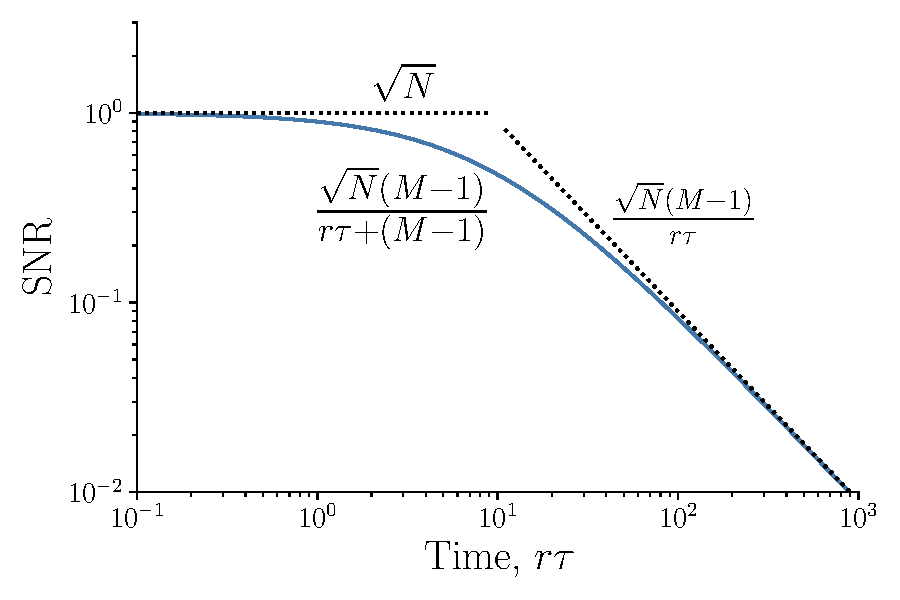
\includegraphics[width=0.4\linewidth]{LenvProven.pdf}}\label{fig:provengen}
  \item\aligntop{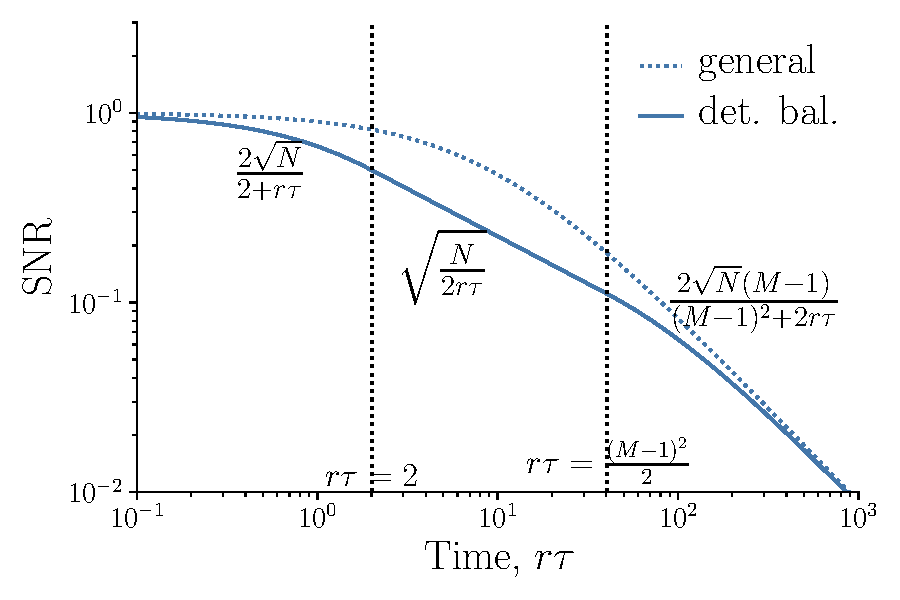
\includegraphics[width=0.4\linewidth]{LenvConj.pdf}}\label{fig:provendetbal}
  \end{myenuma}
  \caption[Proven envelope for the signal-to-noise ratio]
  {(\ref{fig:provengen}) The memory curve envelope that we can prove, \cref{eq:env}.
  (\ref{fig:provendetbal}) Conjectured memory curve envelope when we assume the optimal models satisfy detailed balance, \cref{eq:envDB}.
  The number of synapses \(N=1\) and the number of states \(M=10\).
  The dashed lines indicate the initial SNR bound, \eqref{eq:initbnd}, and the area bound, \eqref{eq:areabnd}, from \cite{Lahiri2013synapse}.}\label{fig:envproven}
\end{figure}

\newcolumntype{B}{R@{\,}C@{\,}L}
% \(
\begin{table}[tb]
  \begin{center}
  \begin{tabular}{BACCCCCC}
    \toprule
      \multicolumn{5}{c}{Domain of validity} & \CI_a & \tau_a 
        & \mu_\CI & \mu_a & \mu_\CA 
        % & \snrb(\tau) 
      \\
    \midrule
      0 &\leq r \tau &\leq 2 & M &\geq 3 & 1 & 2 
        & \frac{4 - 2r \tau}{[2 + r \tau]^2} & \frac{2\sqrt{2}r\tau}{[2 + r \tau]^2} & 0 
        % & \frac{2 \sqrt{N}}{2 + r \tau} 
      \\
      2 &< r \tau &< \frac{(M-1)^2}{2} & M &> 3 & \sqrt{\frac{2}{\tau}} & \tau 
        & 0 & \frac{1}{2\sqrt{r \tau}} & 0 
        % & \sqrt{\frac{N}{2 r \tau}} 
      \\ \addlinespace[0.2ex]
      \frac{(M-1)^2}{2} &\leq r \tau & & M &\geq 3 & \frac{2}{M-1} & \frac{(M-1)^2}{2} 
        & 0 & \frac{\sqrt{2}(M-1)^3}{[(M-1)^2 + 2r \tau]^2} 
        & \frac{4r \tau - 2(M-1)^2}{[(M-1)^2 + 2r \tau]^2} 
        % & \frac{2 \sqrt{N} (M-1)}{(M-1)^2 + 2r \tau} 
      \\
      &-& & M &\leq 3 & 1 & M - 1 
        & \frac{(M-1)^2}{[(M-1) + r \tau]^2} %- \frac{\mu_a \sqrt{\tau_a}}{2} 
        & 0 & \frac{r \tau}{[(M-1) + r \tau]^2} %- \frac{\mu_a}{2 \sqrt{\tau_a}} 
        % & \frac{\sqrt{N} (M-1)}{(M-1) + r \tau} 
      \\
    \bottomrule
  \end{tabular}
  \end{center}
\caption{The solution to the maximum SNR \cref{eq:envKTcond} for the Lagrangian in \cref{eq:envDBlagrangian}, under different conditions. 
The resulting envelope is \cref{eq:envDB}.
The range of \(\tau\) for the second row does not exist for \(M = 3\), in which case any of the other rows can be used.}
\label{tab:envDB}
\end{table}
% \)

%================================================================================

\section{Finite time}\label{sec:finite}

Now we'll maximise \(\snrb(\tau)\) for some fixed \(\tau\), subject to the constraints \eqref{eq:constr}.
First, we will maximise the numerator of \eqref{eq:lsnr} holding \(\eq\w\) fixed.
We can maximise the ration \wrt \(\eq\w\) later.
From this point on, we work in units where \(r = 1\).

Consider the Lagrangian
%
\begin{equation}\label{eq:finitelagrangian}
\begin{aligned}
  \CL =&\, \sum_{ij} \eqm_i \encm_{ij} (\etwm_i(s) - \etwm_j(s))
        +\sum_{\nu i j} \prn{ f^\nu \mu^\nu_{ij} \MMdm^\nu_{ij} }
        &+ \lambda \prn{ \Delta\pr - \sum_i \eqm_i \wm_i },
\end{aligned}
\end{equation}
%
where \(\Delta\pr\) is the constant value we are holding \(\eq\w\) at.
The Karush-Kuhn-Tucker necessary conditions for a maximum are
%
\begin{equation}\label{eq:KTfinite}
  \pdiff{\CL}{\MMdm^\nu_{ij}} = 0, \quad
  \mu^\nu_{ij} \geq 0, \quad
  \pdiff{\CL}{\mu^\nu_{ij}} \geq 0, \quad
  \mu^\nu_{ij}\pdiff{\CL}{\mu^\nu_{ij}} = 0, \quad
  \pdiff{\CL}{\lambda} = 0.
\end{equation}
%
We have scaled the KKT multipliers by \(f^\nu\) for later convenience.

The derivatives, for \(m \neq n\) are
%
\begin{equation}\label{eq:finitederivs}
\begin{aligned}
  \frac{1}{f^\nu} \pdiff{\CL}{\MMdm^\nu_{mn}} = & \,
    \eqm_m \prn{ \brk{\thbm_m(s) - \thbm_n(s)}
     + \prn{\mathbf{c}_m(s) + (-1)^\nu} \brk{\etwm_m(s) - \etwm_n(s)} } \\
     &+ \mu^\nu_{mn} -  \mu^\nu_{mm}
     + \lambda \eqm_m (\etwm_{m}(0)-\etwm_{n}(0)) 
    = 0.
\end{aligned}
\end{equation}
%
We can solve for the KKT multipliers by noting that
%
\begin{equation*}
  \mu^\nu_{ij} \MMdm^\nu_{ij} = 0,
  \qquad \text{and} \qquad
  \sum_{j: j \neq i} \mu^\nu_{ii} \MMdm^\nu_{ij} 
      = \mu^\nu_{ii} (1 - \MMdm^\nu_{ii}) = \mu^\nu_{ii}.
\end{equation*}
%
Then, with some new vectors defined:
%
\begin{equation}\label{eq:kktsol}
\begin{aligned}
  \mu^\nu_{mm} &= - \eqm_m \prn{ \albm^\nu_m(s) 
    + \lambda \ombm^\nu_m(0) 
    + \prn{{c}_m(s) + (-1)^\nu} \ombm^\nu_m(s)
    }, \\
  \mu^\nu_{mn} &= \eqm_m \big( 
      \brk{ \thbm_n(s) - \thbm_m(s) - \albm^\nu_m(s) }
    + \lambda \brk{ \etwm_n(0) - \etwm_m(0) - \ombm^\nu_m(0) } 
  \\ &\phantom{= \eqm_m \big( }
    + \brk{{c}_m(s) + (-1)^\nu} 
        \brk{ \etwm_n(s) - \etwm_m(s) - \ombm^\nu_m(s) }
     \big), \\
  &\text{where} \quad 
  \alb^\nu(s) = (\MMd^\nu - \I) \thb(s), \qquad
  \omb^\nu(s) = (\MMd^\nu - \I) \etw(s).
\end{aligned}
\end{equation}
%

The expressions in \cref{eq:finitederivs} have the same form as for \(s=0\), which allowed us to argue that the model with maximal area must have the serial topology, \cite{Lahiri2013synapse}.
The one missing ingredient is the scale invariance.

However, we do have numerical evidence that the model that maximises the Laplace transform does have the serial topology.
In \cref{fig:envnum} we see the result of numerical maximisation of \cref{eq:finitelagrangian}.
We see that restricting to the serial topology does not make the performance any worse.
In fact, it slightly improves the performance, but this can be ascribed to the numerical optimisation problem being easier.
Assuming that the optimiser did find the global maximum, this provides evidence for our conjecture that the model that maximises the Laplace transform must have the serial topology.

Note that models with the serial topology must satisfy detailed balance.
Therefore, this conjecture implies that the square-root bound of \cref{sec:sqrt} applies, implying the stricter envelope of \cref{eq:envDB}.
In \cref{fig:envnum}, we can see that this envelope is close to tight, being off by a constant factor.


\begin{figure}[tb]
  \centering
  % Requires \usepackage{graphicx}
  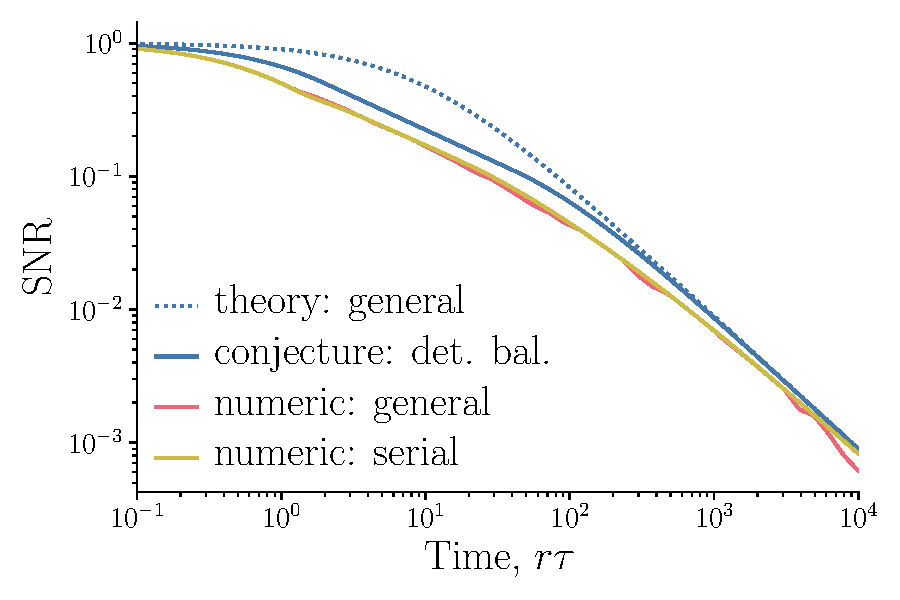
\includegraphics[width=0.8\linewidth]{LenvNum.pdf}\\
  \caption[Numerical envelope for the signal-to-noise ratio]
  {Numerical envelope for the signal-to-noise ratio, \eqref{eq:snrb}. 
  \Cref{eq:finitelagrangian,eq:KTfinite,eq:finitederivs} are solved numericallly with \(f\potdep=\frac{1}{2}\), the number of synapses \(N=1\) and the number of states \(M=10\).
  The orange line indicates maximisation of the memory curve over the space of all matrices satisfying the constraints \eqref{eq:constr}.
  The green line indicates maximisation over models with the serial topology, \ie potentiation only moves up one state and depression only moves down one state.
  The dotted blue line indicates the proven envelope, \cref{eq:env} and the solid blue line is the conjectured envelope assuming detailed balance, see \cref{eq:envDB}.}\label{fig:envnum}
\end{figure}


%-------Section------------------------------------------------------------------

\subsection{Scale invariance}\label{sec:scale}

Under the transformation from \cref{eq:scale}, the Laplace transform has the following scaling property
%
\begin{equation}\label{eq:laplacescale}
  \hat{A} \prn{\zeta s;\zeta * \MMd^\nu} = \hat{A} \prn{s; \MMd^\nu}.
\end{equation}
%
At \(s = 0\), it is scale invariant.
This means that we can take a pair of matrices that violates the ``diagonal'' constraints (second inequality of \eqref{eq:constri}) and use the scale transform \eqref{eq:scale} to construct a pair of matrices that satisfy the ``diagonal'' constraints and have the same area.
This allowed us to ignore the diagonal constraints.
We can't do that for \(s > 0\).

The corresponding symmetry here is scaling the shifted process from \cref{eq:lshiftpd}, which amounts to
%
\begin{equation}\label{eq:shiftscale}
  \zeta {\circledast}_{s} \MMd 
      \equiv \zeta \MMd
      + (1 - \zeta) \brk{(1 + s)\I - s \onev \eq} .
\end{equation}
%
Then we have
%
\begin{equation}\label{eq:lshiftscale}
  \hat{A} \prn{s; \MMd^\nu} 
    = \hat{A} \prn{0, \shift{\MMd}^\nu(s)}
    = \hat{A} \prn{0, \zeta * \shift{\MMd}^\nu(s)}
    = \hat{A} \prn{s, \zeta \circledast_s \MMd^\nu}.
\end{equation}
%
The problem here is that the lower bound, \(\MMdm^\nu_{ij} \geq 0\), 
is not invariant under this transformation, unlike the \(s = 0\) case.
Using this transformation to fix the upper bound can break the lower bound.

We might ask what conditions are required so that a model is fixable?
This means that the \(\zeta \circledast_s \) orbit of the model contains some valid models.
The conditions are
%
\begin{equation*}
\begin{alignedat}{5}
  [\zeta \circledast \MMd^\nu]_{ij}  
    &= \zeta \MMdm^\nu_{ij} - (1-\zeta) s \eqm_j 
    &&\geq 0 &
  \quad &\implies \quad &
  \zeta &\geq \frac{s \eqm_j}{\MMdm^\nu_{ij} + s \eqm_j} &
    &\forall \nu, i, j : i \neq j , \\
  \sum_{j : i \neq j} [\zeta \circledast \MMd^\nu]_{ij} 
    &= \zeta \lbm^\nu_i - (1-\zeta) s (1-\eqm_i) 
    &&\leq 1 &
  &\implies &
  \zeta &\leq \frac{1 + s (1-\eqm_i)}{\lbm^\nu_i + s (1-\eqm_i)} &
    \quad &\forall \nu, i ,
\end{alignedat}
\end{equation*}
%
where \(\lbm^\nu_i \equiv \sum_{j : i \neq j} \MMdm^\nu_{ij}\) is the inverse mean  lifetime of state \(i\).
The model is fixable if it is possible to find a \(\zeta\) that satisfies all of the above conditions:
%
\begin{equation}\label{eq:fixable}
  \frac{s \eqm_j}{\MMdm^\nu_{ij} + s \eqm_j} \leq \frac{1 + s (1-\eqm_k)}{\lbm^\mu_k + s (1-\eqm_k)}
  \quad \implies \quad
  \frac{\lbm^\mu_k - 1}{1 + s (1-\eqm_k)} \leq \frac{\MMdm^\nu_{ij}}{s \eqm_j} 
  \quad \forall \mu, \nu, i, j, k : i \neq j.
\end{equation}
%
Note that when \(\MMdm^\nu_{ij} = 0\) for some \(i,j \), this condition reduces to \(\lbm^\mu_k \leq 1\), the original diagonal constraint.
Thus, relaxing the constraints from ``the model is valid'' to ``the model is fixable'' doesn't help us prove anything about the topology.


%-------Section------------------------------------------------------------------

\subsection{Shifted problem}\label{sec:lshift}

The relation of the Laplace transform to the shifted process from \cref{eq:lshiftpd,eq:lareashift} suggests an alternative approach: 
treat the off-diagonal components of \(\shift{\MMd}^\nu \) as the degrees of freedom and maximise the area instead.
The constraints on \(\shift{\MMdm}^\nu_{ij}\) are different from \cref{eq:constri}:
%
\begin{equation}\label{eq:lshiftconstr}
  \shift{\MMdm}^\nu_{ij} \geq s \eqm_j,
    \quad \forall \; \nu, i, j : i \neq j, \qquad
  \sum_{j: j \neq i} \shift{\MMdm}^\nu_{ij} \leq 1 + s (1 - \eqm_i).
    \quad \forall \; \nu, i.
\end{equation}
%
The diagonal elements are still given by \( \shift{\MMdm}^\nu_{ii} = 1 - \sum_{j: j \neq i} \shift{\MMdm}^\nu_{ij} \), but now they are allowed to be negative so long as \(\shift{\MMdm}^\nu_{ii} \geq - s (1 - \eqm_i)\).

The Lagrangian we should consider is
%
\begin{equation}\label{eq:lshiftlagrangian}
\begin{aligned}
  \CL =&\, \sum_{ij} \eqm_i \encm_{ij} (\etwm_i - \etwm_j)
        +\sum_{\nu i j}  f^\nu \mu^\nu_{ij}\prn{\MMdm^\nu_{ij} -  s (\eqm_j - \delta_{ij}) }
        &+ \lambda \prn{ \Delta\pr - \sum_i \eqm_i \wm_i },
\end{aligned}
\end{equation}
%
where all of the first-passage times are evaluated at \(s = 0\).

In \cref{fig:shifted} we show the result of solving this problem with numerical optimisation.
We see essentially the same results as the original problem, \cref{eq:finitelagrangian,fig:envnum}, as expected.

The derivatives, for \(m \neq n\) are
%
\begin{equation}\label{eq:lshiftderivs}
\begin{aligned}
  \frac{1}{f^\nu} \pdiff{\CL}{\MMdm^\nu_{mn}} = & \,
    \eqm_m \prn{ \brk{\thbm_m - \thbm_n}
     + \prn{{c}_m + (-1)^\nu + \lambda} \brk{\etwm_m - \etwm_n} } \\
     &+ \mu^\nu_{mn} -  \mu^\nu_{mm}
     - \sum_{ij} \mu^\nu_{ij} s f^\nu \eqm_m (\fptbm_{mj} - \fptbm_{nj}) \eqm_j
    = 0.
\end{aligned}
\end{equation}
%
We can absorb the new terms by defining
%
\begin{equation*}
\begin{aligned}
  \shift{\thb}^\nu(s) = \thb(0) - s f^\nu \fptb(0) \Eq (\boldsymbol{\mu}^\nu)\trans \onev,
  \qquad
  \shift{\alb}^\nu(s) &= (\MMd^\nu + (s - 1) \I - s \onev \eq) \shift{\thb}^\nu(s),
  \\
  \shift{\omb}^\nu(s) &= (\MMd^\nu + (s - 1) \I - s \onev \eq) \etw(0).
\end{aligned}
\end{equation*}
%
We note that
%
\begin{equation*}
  \mu^\nu_{ij} (\MMdm^\nu_{ij} - s \eqm_j) = 0,
  \qquad \text{and} \qquad
  \sum_{j: j \neq i} \mu^\nu_{ii} (\MMdm^\nu_{ij} - s \eqm_j)
      = \mu^\nu_{ii} (1 - \MMdm^\nu_{ii} - s (1 - \eqm_i)) = \mu^\nu_{ii},
\end{equation*}
%
then we can ``solve'' for the KKT multipliers:
%
\begin{equation}\label{eq:lshiftsol}
\begin{aligned}
  \mu^\nu_{mm} &= - \eqm_m \prn{ \shift{\albm}^\nu_m(s) 
    + \brk{ {c}_m + (-1)^\nu + \lambda } \shift{\ombm}^\nu_m(s)
    }, \\
  \mu^\nu_{mn} &= \eqm_m \prn{ 
      \brk{ \shift{\thbm}^\nu_n(s) - \shift{\thbm}^\nu_m(s) - \shift{\albm}^\nu_m(s) }
  % \\ & \phantom{= - \eqm_m \big( } 
    + \brk{ {c}_m + (-1)^\nu + \lambda } 
        \brk{ \etwm_n - \etwm_m - \shift{\ombm}^\nu_m(s) }
     }, \\
\end{aligned}
\end{equation}
%
although there are KKT multipliers hiding in \(\shift{\thb}^\nu(s)\) and \(\shift{\alb}^\nu(s)\).

While this problem involves the scale invariant quantity \(\hat{A}(0)\), neither the upper nor lower bounds in \cref{eq:lshiftconstr} are invariant.
We then run into the same problems in proving our serial-topology hypothesis.

\begin{figure}[ht]
\begin{center}
\begin{myenuma}
  \item \aligntop{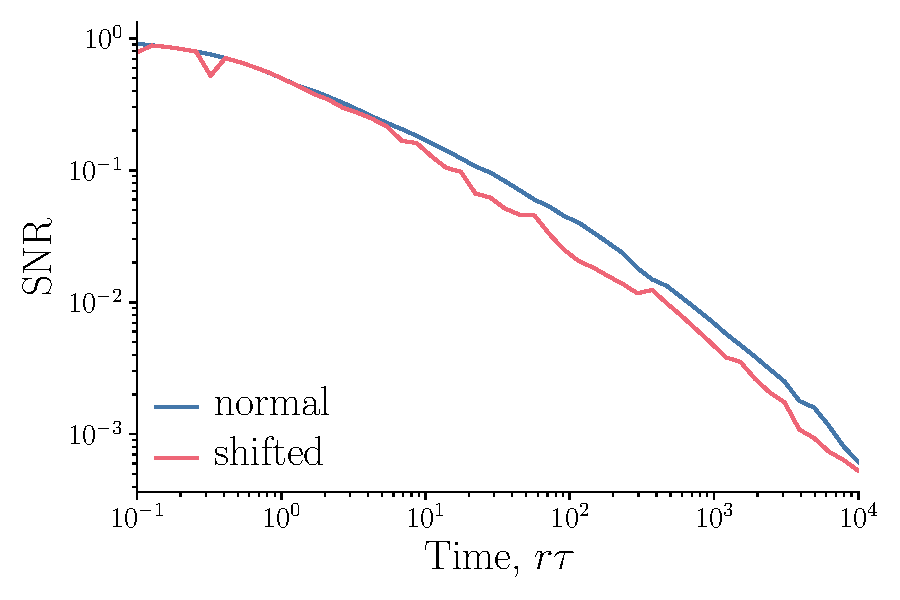
\includegraphics[width=0.4\linewidth]{LenvShift.pdf}}
  \label{fig:envshift}
  \item \aligntop{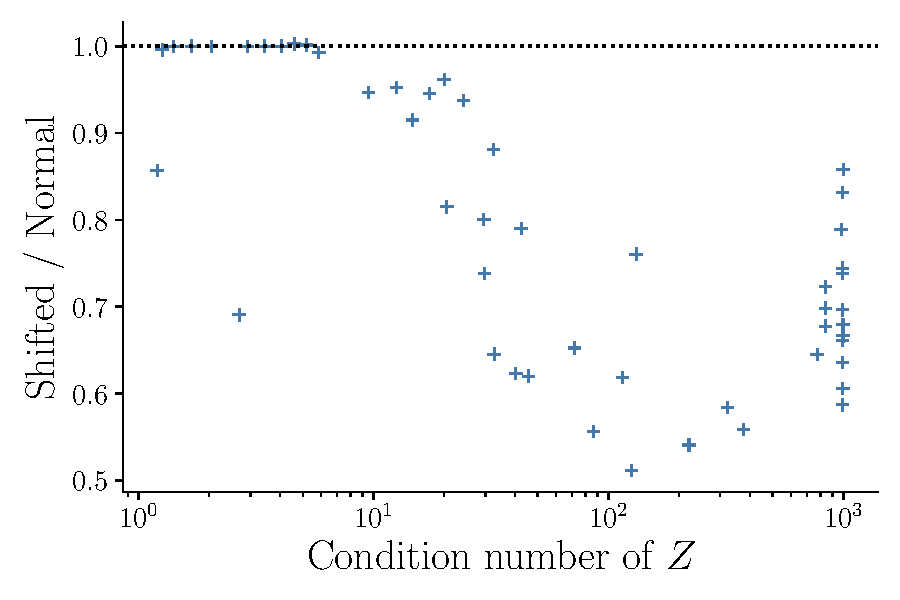
\includegraphics[width=0.4\linewidth]{shift_cond.pdf}}
  \label{fig:shiftcond}
\end{myenuma}
\caption[Shifted problem vs.\ original]{Shifted problem vs.\ original.
(\ref*{fig:envshift}) Comparison of numerical optimisation of the shifted problem in \cref{eq:lshiftlagrangian,fig:envnum} with the original problemin \cref{eq:finitelagrangian}.
We see that the two approaches produce very similar numerical envelopes.
The shifted problem involves non-linear constraints and is thus harder to solve.
(\ref{fig:shiftcond}) Plot of the discrepancy in (\ref*{fig:envshift}) against the condition number of the fundamental matrix, \(\fund \).
We see that most of the large discrepancies occur where the problem is numerically ill-conditioned.
\label{fig:shifted}}
\end{center}
\end{figure}

\begin{figure}[tbp]
  \centering
  % Requires \usepackage{graphicx}
  \begin{myenuma}
  \item\aligntop{\includegraphics[width=0.45\linewidth,page=7]{envelope.pdf}}
  \item\aligntop{\includegraphics[width=0.45\linewidth,page=13]{envelope.pdf}}
  \item\aligntop{\includegraphics[width=0.45\linewidth,page=21]{envelope.pdf}}
  \item\aligntop{\includegraphics[width=0.45\linewidth,page=27]{envelope.pdf}}
  \item\aligntop{\includegraphics[width=0.45\linewidth,page=36]{envelope.pdf}}
  \item\aligntop{\includegraphics[width=0.45\linewidth,page=50]{envelope.pdf}}
  \end{myenuma}
  \caption[Optimal models]{The models that constitute the numeric envelope in \autoref{fig:envnum}.
  The plot to the left of each frame indicates the memory curve of the model shown to the right in green, with the numeric envelope for models with the serial topology in orange and the proven envelope, \eqref{eq:env}, in blue.
  Above the left plot we have a graphical display of the model, described with more detail to the right.
  The area of each node is proportional to the steady state probability in that state and the thickness of the red and blue edges are proportional to the transition probabilities under potentiation and depression.
  The bar graph in the upper right of each frame indicates the transition probabilities from the state to the left of each bar to the state on its right, under potentiation.
  The bar graph in the lower right of each frame indicates the transition probabilities from the state to the right of each bar to the state on its left, under depression.
  The heat map in the centre right of each frame indicates the equilibrium probability distribution for each state.
  See the video for the full set of models.}\label{fig:envvid}
\end{figure}

%================================================================================

\section{Nearly uniform serial models}\label{sec:serial}

\begin{figure}[tb]
  \centering
  % Requires \usepackage{graphicx}
  \begin{myenuma}
    \item\aligntop{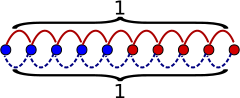
\includegraphics[width=0.26\linewidth]{serial_uni.svg}}\hspace{0.02\linewidth}\label{fig:serial_uniform}
    \item\aligntop{\includegraphics[width=0.26\linewidth]{serial_sticky.svg}}\hspace{0.02\linewidth}\label{fig:serial_sticky}
    \item\aligntop{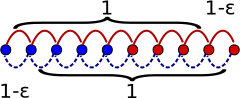
\includegraphics[width=0.26\linewidth]{serial_shorten.svg}}\label{fig:serial_shorten}
  \end{myenuma}
  \caption[Heuristic optimal models]{Heuristics for models that maximise memory curve.
  All unlabelled arrowshave transition probabilities equal to 1.
  At one particular time, the model is (\ref{fig:serial_uniform}) the uniform serial model with \(M\) states.
  At later times, the model has (\ref{fig:serial_sticky}) ``sticky'' end states with low exit transition probabilities, tending to the area maximising model.
  At earlier times, the model is (\ref{fig:serial_shorten}) progressively shortened by reducing the transition probability to the end states.
  Once this reaches zero, we discard the old end state and work on the new end state.} \label{fig:heuristicmodels}
\end{figure}


Looking at them models that were found by numerical maximisation in \autoref{fig:envvid} (see the video for the full set of models), suggests we look at the particular set of models, shown in \autoref{fig:heuristicmodels}.

At one particular time, the model is (\ref{fig:serial_uniform}) the uniform serial model with \(M\) states.
At later times, the model has (\ref{fig:serial_sticky}) ``sticky'' end states with low exit transition probabilities, tending to the area maximising model as \(\tau \to \infty\).
At earlier times, the model is (\ref{fig:serial_shorten}) progressively shortened by reducing the transition probability to the end states.
Once this reaches zero, we discard the old end state and shorten further by reducing the transition probability to the new end state (as one can see from \autoref{fig:envvid} and the video, this is not quite true, but it is close enough to true to get a reasonable approximation to the envelope).
Once the length has been reduced to \(M=2\), the model is not shortened any further and the two-state model with deterministic transitions maximises the memory curve for all earlier times.

These models' Laplace transforms can be computed analytically, as we will see below, leading to a heuristic envelope.
All of these calculations will be performed at \(f\potdep=\frac{1}{2}\), so the denominator will play no role.
We will work in units such that \(r=1\) temporarily, only restoring \(r\) at the end.
We study models with \(m\) strong and \(m\) weak states for a total of  \(M = 2 m\).

%--------------------------------------------------------------------------------

\subsection{Uniform serial model}\label{sec:serial_uniform}


Here we will look at the model in \autoref{fig:heuristicmodels}\ref{fig:serial_uniform}.
Looking at \eqref{eq:larea}, the only thing we need is differences in \(\etwm_i(s)\).
In fact, given that the only nonzero elements of \(\enc\) are
%
\begin{equation}\label{eq:unienc}
  \encm_{ii+1}=\frac{1}{2} \quad\text{for}\quad i<2m,
  \qquad
  \encm_{ii-1}=-\frac{1}{2} \quad\text{for}\quad i>1,
\end{equation}
%
and \(\eqm_i = \frac{1}{2m}\), we have
%
\begin{equation}\label{eq:uniareaeta}
  \hat{A}(s) = \frac{\etwm_1(s) - \etwm_{2m}(s)}{2m}.
\end{equation}
%

Note that
%
\begin{equation}\label{eq:etafund}
  \etw(s) = \text{const.} - \fund(s)\w.
\end{equation}
%
As we are only interested in differences of the \(\etwm_i(s)\), we can drop the constant.
Then
%
\begin{equation}\label{eq:etarecur}
  -(s\I + \onev\pib - \frg)\etw(s) = \w.
\end{equation}
%
We can then write
%
\begin{equation}\label{eq:detarecur}
  \etw(s) = -\frac{(\pib\etw(s))\onev+\w}{s} + \delta \boldsymbol{\eta}(s),
  \qquad
  (\frg-s\I)\delta \boldsymbol{\eta}(s) = \frac{\frg\w}{s}.
\end{equation}
%
As we are only interested in differences, we can drop any terms proportional to \(\onev\) in \(\etw(s)\).

The \(i\)'th row of this equation reads
%
\begin{equation}\label{eq:detarow}
  \frac{\delta\eta_{i+1}+\delta\eta_{i-1}}{2} - (s+1)\delta\eta_i = 0,
\end{equation}
%
with the following exceptions
%
\begin{equation}\label{eq:detabnduni}
\begin{aligned}
  \frac{\delta\eta_2}{2} - \prn{s+\frac{1}{2}}\delta\eta_1 &= 0, \\
  \frac{\delta\eta_{m+1}+\delta\eta_{m-1}}{2} - (s+1)\delta\eta_{m} &= \frac{1}{s},\\
  \frac{\delta\eta_{m+2}+\delta\eta_{m}}{2} - (s+1)\delta\eta_{m+1} &= -\frac{1}{s},\\
  \frac{\delta\eta_{2m-1}}{2} - \prn{s+\frac{1}{2}}\delta\eta_{2m} &= 0.
\end{aligned}
\end{equation}
%
These equations are invariant under \(\delta\eta_{2m+1-i} \to -\delta\eta_i\), so these two must be equal.
Then we have
%
\begin{equation}\label{eq:detahalf}
\begin{aligned}
  \frac{\delta\eta_{i+1}+\delta\eta_{i-1}}{2} - (s+1)\delta\eta_i &= 0,
  \quad\text{for}\quad 1<i<m, \\
  \frac{\delta\eta_2}{2} - \prn{s+\frac{1}{2}}\delta\eta_1 &= 0, \\
  \frac{\delta\eta_{m-1}}{2} - \prn{s+\frac{3}{2}}\delta\eta_{m} &= \frac{1}{s}.
\end{aligned}
\end{equation}
%

The first of these equations is solved by
%
\begin{equation}\label{eq:detagensol}
  \delta\eta_i = B\e^{\beta(i-1)} + C\e^{\beta(1-i)},
  \qquad\text{where}\qquad
  s = S(\beta) \equiv 2 \sinh^2 \prn{\frac{\beta}{2}}
    = \cosh (\beta) - 1,
\end{equation}
%
with \(B\) and \(C\) determined by the boundary conditions provided by the last two equations of \eqref{eq:detahalf}:
%
\begin{equation}\label{eq:unicoeffs}
  B = -\frac{1}{s(1 + \e^{-\beta}) \cosh \prn{m \beta}},
  \qquad
  C = -\frac{1}{s(\e^{\beta} + 1) \cosh \prn{m \beta}}.
\end{equation}
%
This can be used to compute the Laplace transform
%
\begin{equation}\label{eq:unilaplace}
  A(s) = \frac{\etwm_1(s)}{m}
   = \frac{1}{m}\prn{\frac{1}{s}+B+C}
   = \frac{2\sinh^2\prn{\frac{m \beta}{2}}}{m s \cosh\prn{m \beta}}
   = \frac{2 S\prn{m \beta}}{M s \prn{S\prn{m \beta} + 1}}.
\end{equation}
%

In reality, \(M\) can only take even integer values.
However, one can find a heuristic approximation to the envelope by maximising \wrt \(M\).
We find that
%
\begin{multline}\label{eq:unienv}
  M_* = \pm\frac{2y_*}{\beta},
  \quad
  s = 2\sinh^2\frac{y_*}{M_*},
  \qquad
  \hat{A}_*(s) = \prn{\frac{ 2\sinh^2 \frac{y_*}{2} }{ y_* \cosh y_* } } \frac{\abs{\beta}}{s},
  \\ \text{where}\quad
  y_* = \tanh \frac{y_*}{2} \cosh y_* \approx 1.50553.
  \qquad
\end{multline}
%
This is only valid for
%
\begin{equation}\label{eq:univalid}
  2 \leq M_* \leq M,
  \qquad\implies\qquad
  2\sinh^2 \frac{y_*}{M} \leq s \leq 2\sinh^2 \frac{y_*}{2}.
\end{equation}
%
When \(M \gg 2\), the validity region is approximately
%
\begin{equation}\label{eq:univalidapprox}
  \frac{4.53327}{M^2} \lesssim s \lesssim 1.36423.
\end{equation}
%
When \(s \sim \CO(M^{-2}) \ll 1\), we have \(\beta \approx \pm \sqrt{2s}\) and the heuristic envelope is approximately
%
\begin{equation}\label{eq:unienvapprox}
  \hat{A}_*(s) \approx \frac{ 0.54203 }{ \sqrt{s} }.
\end{equation}
%
We will lok at a more accurate interpolation between different \(M\) in the \hyperref[sec:serial_shorten]{next section}.

For \(s\gtrsim 1.36423\), we set \(M=2\) to find
%
\begin{equation}\label{eq:binaryenv}
  \hat{A}(s) = \frac{1}{1+s}.
\end{equation}
%
This does not match up with \eqref{eq:unienvapprox} at the boundary of the two regions, as this is outside the regime of validity of that approximation.
However, it does match up with the full formula, \eqref{eq:unienv} at the boundary.

%--------------------------------------------------------------------------------

\subsection{Shortened serial model}\label{sec:serial_shorten}


Here we will look at the model in \autoref{fig:heuristicmodels}\ref{fig:serial_shorten}.
We proceed in the same manner as in \autoref{sec:serial_uniform}, with the following differences.

The following elements of \(\enc\) and \(\eq\) differ from \eqref{eq:unienc}:
%
\begin{equation}\label{eq:shortenenc}
  \begin{aligned}
  \encm_{2m-1,2m} = -\encm_{2,1} &= \frac{(1-\varepsilon)}{2},
  &\qquad
  \eqm_1 = \eqm_M &= \frac{(1-\varepsilon)}{2(m-\varepsilon)},
  \\ &&
  \eqm_i &=  \frac{1}{2(m-\varepsilon)}
  \quad\text{for}\quad 1<i<2m.
  \end{aligned}
\end{equation}
%
This means that the Laplace transform is given by
%
\begin{equation}\label{eq:shortenareaeta}
  \hat{A}(s) = \frac{(1-\varepsilon)(\etwm_1(s)-\etwm_{2m}(s)) 
                      + \varepsilon(\etwm_2(s)-\etwm_{2m-1}(s))}
                    {2(m-\varepsilon)}
       = \frac{2(1-\varepsilon) \etwm_1(s) + 2\varepsilon\,\etwm_2(s)}
              {2(m-\varepsilon)}.
\end{equation}
%

The \(\etwm_i(s)\) take the same general form \eqref{eq:detagensol} except for \(i=1\), and with different coefficients due to the different boundary conditions
%
\begin{equation}\label{eq:detabndshorten}
\begin{aligned}
  \frac{\delta\eta_2}{2} - \prn{s+\frac{1}{2}}\delta\eta_1 &= 0, \\
  \frac{\delta\eta_3 + (1-\varepsilon)\delta\eta_1}{2} - \prn{s+\frac{2-\varepsilon}{2}}\delta\eta_2 &= 0, \\
  \frac{\delta\eta_{m-1}}{2} - \prn{s+\frac{3}{2}}\delta\eta_{m} &= \frac{1}{s}.
\end{aligned}
\end{equation}
%
These are solved by
%
%
\begin{equation}\label{eq:shortensol}
\begin{aligned}
  \delta\eta_i &= B\e^{(i-2)\beta} + C\e^{(2-i)\beta} \qquad
        \text{for} \quad 2 \leq i \leq m, \\
  \delta\eta_1 &= \frac{1}
         {[(1-\varepsilon)\cosh(m\beta) + \varepsilon(2s+1)\cosh((m-1)\beta)]s}, \\
  B &= - \frac{(2s+1) \e^{\beta/2} + (1-\varepsilon) \tanh(\beta/2)}
         {s [(1-\varepsilon)\cosh(m\beta) + \varepsilon(2s+1)\cosh((m-1)\beta)]}, \\
  C &= - \frac{((2s+1) \e^{-\beta/2} - (1-\varepsilon) \tanh(\beta/2)}
         {s [(1-\varepsilon)\cosh(m\beta) + \varepsilon(2s+1)\cosh((m-1)\beta)]}, \\
\end{aligned}
\end{equation}
%
Which gives the following Laplace transform
%
\begin{equation}\label{eq:shortenlaplace}
  \hat{A}(s) = \frac{(1-\varepsilon) S(m\beta) + \varepsilon(2s+1) S((m-1)\beta)}
          { s [m-\varepsilon]
            [(1-\varepsilon)[S(m\beta) + 1] + \varepsilon(2s+1)[S((m-1)\beta) + 1]] }.
\end{equation}
%
This interpolates between \eqref{eq:unilaplace} at \(\varepsilon=0\) and the same expression for \(m-1\) at \(\varepsilon=1\).

This expression breaks down for \(M = 2\), as there are no \( 2 \leq i \leq m \) when \(m = 1\).
In that case, 
%
\begin{equation}\label{eq:binaryshorten}
  \hat{A}(s) = \frac{1-\varepsilon}{1-\varepsilon + s}.
\end{equation}
%
We can see that the optimal \(\varepsilon = 0\), reducing \cref{eq:binaryshorten} to \cref{eq:binaryenv}.

To find the optimal \(\varepsilon\) at any given \(s\), it helps if we define
%
\begin{equation*}
\begin{aligned}
  \Delta f_m(\beta) &= S(m\beta) - \zeta S((m-1)\beta), &
  f_m(\beta) &= \frac{S(m\beta)}{\Delta f_m(\beta)}, \\
  \Delta g_m(\beta) &= \Delta f_m(\beta) + 1 - \zeta , &
  g_m(\beta) &= \frac{S(m\beta) + 1}{\Delta g_m(\beta)}, \\
  \text{where}\quad \zeta &= 2s + 1, 
  \qquad\qquad \implies & 
  \hat{A}(s) &= \frac{\Delta f_{m} (f_m - \varepsilon)}
           {s \Delta g_{m} (m - \varepsilon) (g_m - \varepsilon)}.
  \\
\end{aligned}
\end{equation*}
%
The results are plotted in \cref{fig:shorten}.

\begin{figure}[ht]
\begin{center}
\begin{myenuma}
  \item\label{fig:short_opt}\aligntop{%
    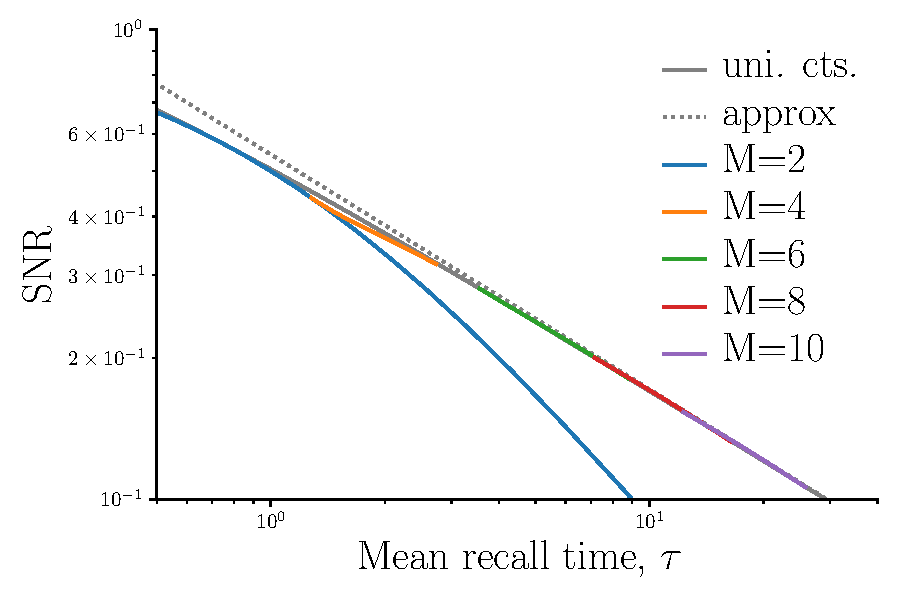
\includegraphics[width=0.45\linewidth]{shorten_opt.pdf}}
  \item\label{fig:short_ratio}\aligntop{%
    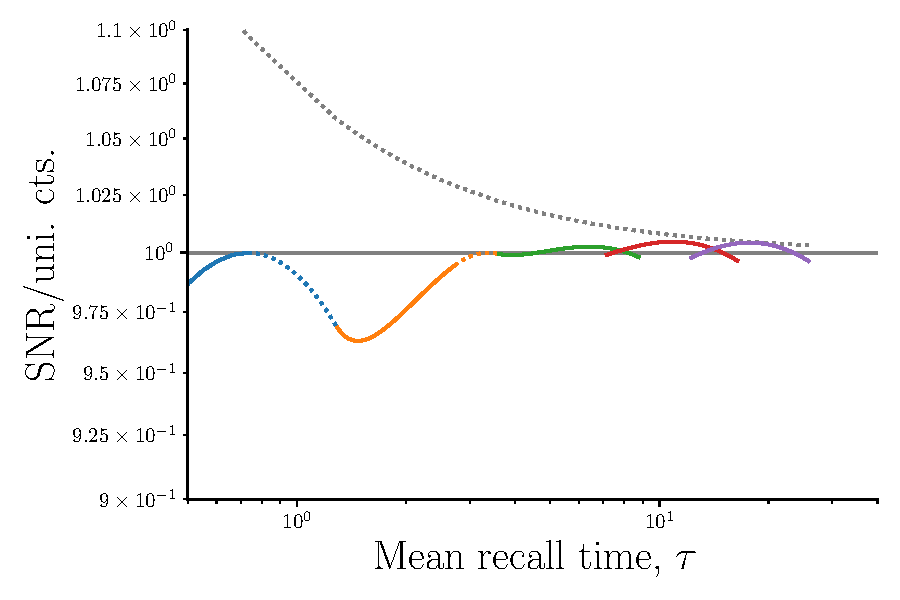
\includegraphics[width=0.45\linewidth]{shorten_ratio.pdf}}
\end{myenuma}
\caption[Signal-to-noise ratio for optimal shortened models]
{Signal-to-noise ratio for optimal shortened models, \cref{eq:shortenenc} optimised over \(\varepsilon\).
(\ref{fig:short_opt}): Solid grey line is \cref{eq:unienv}, the uniform model with \(M\) treated as a continuous parameter and optimised.
Dotted grey line is the approximate expression from \cref{eq:unienvapprox}.
The other curves are from \cref{eq:shortopt}, optimised shortened models for various values of \(M\).
(\ref{fig:short_ratio}): The ratios of the quantities plotted in (\ref{fig:short_opt}) to \cref{eq:unienv}.
The dotted blue and orange lines are the extensions of the \(M=2,4\) lines with \(\varepsilon\) held at 0, as discussed below \cref{eq:shortenvalid}.
Noting the scale of the y-axis, we see that \cref{eq:unienv,eq:unienvapprox} do provide good approximations, especially for larger \(M\).
\label{fig:shorten}}
\end{center}
\end{figure}

We can maximise this \wrt \(\varepsilon\), which yields
%
\begin{equation}\label{eq:shortopt}
  (\varepsilon - f_m)^2 = (m - f_m)(g_m - f_m),
  \quad \implies \quad
  \hat{A}(s) = \frac{\Delta f_{m}}
      {s \Delta g_{m} \brk{\sqrt{\abs{m - f_m}} - \sqrt{\abs{g_m - f_m}}}^2}.
\end{equation}
%
We can find the boundary of the region of applicability by asking at what value of \(s\) is the optimal value of \(\varepsilon=0\) or \(1\)?
%
\begin{equation}\label{eq:shortenvalid}
\begin{aligned}
  \left.\pdiff{\hat{A}(s)}{\varepsilon}\right|_{\mathrlap{\varepsilon=0}} \propto &\,
    m \zeta \brk{S(m\beta) - S((m-1)\beta)} - S(m\beta) [S(m\beta) + 1]
      = 0,\\
  \left.\pdiff{\hat{A}(s)}{\varepsilon}\right|_{\mathrlap{\varepsilon=1}} \propto &\,
    (m-1)\brk{S(m\beta) - S((m-1)\beta)} - \zeta S((m-1)\beta) [S((m-1)\beta) + 1]
      = 0,\\
    &\text{where}\quad
    \zeta = 2s + 1, \qquad
    s = S(\beta) = 2 \sinh^2(\beta/2),
\end{aligned}
\end{equation}
%
with the \(\varepsilon=0\) case providing the lower boundary and \(\varepsilon=1\) providing the upper boundary.
For lower \(s\), \(\varepsilon = 0\) is the optimum. 
For higher \(s\), \(\varepsilon = 1\) is the optimum, which is eqivalent to \(\varepsilon = 0\) with \(M-2\) states.
This is depicted by the dotted lines in \cref{fig:shorten}\ref{fig:short_ratio}.

\(M=2\) is a special case:
%
\begin{equation*}
  \hat{A}(s) = \frac{(\alpha-1)^2}
                    {[2(\alpha^2-\alpha+1) - (1-\varepsilon) (\alpha-1)^2]s},
\end{equation*}
%
so \(\varepsilon=0\) is always the maximum.

If these were really the models that maximised \(A(s)\), the region of validity for \(M\) would not overlap with that for \(M-2\).
In fact there are overlaps, as seen in \cref{fig:shorten}\ref{fig:short_ratio} for \(M=6\) and higher.
This is related to the fact that \autoref{fig:envvid} and the video shows that the optimal models do not shorten by one state at a time, but several outgoing transition probabilities are reduced at once.

%--------------------------------------------------------------------------------

\subsection{Sticky serial model}\label{sec:serial_sticky}

Here we will look at the model in \autoref{fig:heuristicmodels}\ref{fig:serial_sticky}.
We proceed in the same manner as in \autoref{sec:serial_uniform}, with the following differences.

The following elements of \(\enc\) and \(\eq\) are differ from \eqref{eq:unienc}:
%
\begin{equation}\label{eq:stickyenc}
  \begin{aligned}
  \encm_{1,2} = -\encm_{2m,2m-1} &= \frac{1-\varepsilon}{2},
  &\quad
  \eqm_1 = \eqm_{2m} &= \frac{1}{2(m-(m-1)\varepsilon)},
  \\ &&
  \eqm_i &=  \frac{1-\varepsilon}{2(m-(m-1)\varepsilon)}
  \quad\text{for}\quad 1<i<2m.
  \end{aligned}
\end{equation}
%
This means that the Laplace transform is given by
%
\begin{equation}\label{eq:stickyareaeta}
  \hat{A}(s) = \frac{(1-\varepsilon)(\etwm_1(s)-\etwm_M(s))}
                    {2(m-(m-1)\varepsilon)}
       = \frac{2(1-\varepsilon)\, \etwm_1(s)}{2(m-(m-1)\varepsilon)}.
\end{equation}
%

The \(\etwm_i(s)\) take the same general form \eqref{eq:detagensol}, but with different coefficients due to the different boundary conditions
%
\begin{equation}\label{eq:detabndsticky}
\begin{aligned}
  \frac{\varepsilon\delta\eta_2}{2} - \prn{s+\frac{1-\varepsilon}{2}}\delta\eta_1 &= 0, \\
  \frac{\delta\eta_{m-1}}{2} - \prn{s+\frac{3}{2}}\delta\eta_{m} &= \frac{1}{s}.
\end{aligned}
\end{equation}
%
These are solved by
%
\begin{equation}\label{eq:stickycoeffs}
\begin{aligned}
  B &= -\frac{\e^{\beta} - \varepsilon}
      {s [\e^{\beta} + 1] [\cosh(m\beta) - \varepsilon \cosh((m-1)\beta)]}, \\
  C &= -\frac{1 - \varepsilon\e^{\beta}}
      {s [\e^{\beta} + 1] [\cosh(m\beta) - \varepsilon \cosh((m-1)\beta)]},
\end{aligned}
\end{equation}
%
which leads to the Laplace transform
%
\begin{equation}\label{eq:stickylaplace}
  \hat{A}(s) = \frac{(1-\varepsilon)}{[m-(m-1)\varepsilon]s} \,
      \brk{\frac{S(m\beta) - \varepsilon S((m-1)\beta)}
      {S(m\beta) - \varepsilon S((m-1)\beta) + 1 - \varepsilon}}.
\end{equation}
%

\begin{figure}[ht]
\begin{center}
  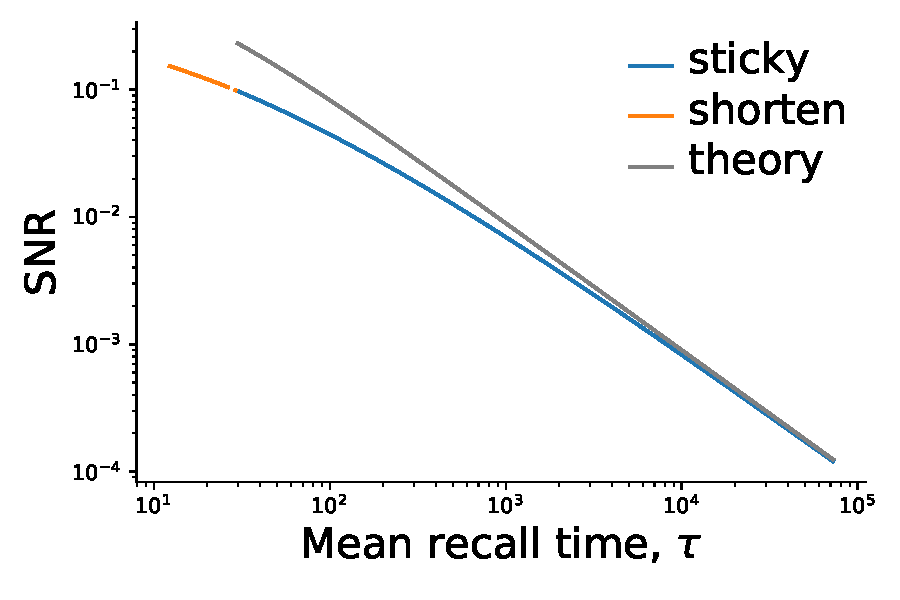
\includegraphics[width=0.4\linewidth]{sticky_opt.pdf}
\caption[Signal-to-noise ratio for optimal sticky models]
{Signal-to-noise ratio for optimal sticky models, \cref{eq:stickyopt} for \(M=10\), in blue.
  The orange line is the SNR for the optimised shortened models, \cref{eq:shortopt} with \(M=10\).
  The grey line is our theoretical envelope from \cref{eq:env}.
  \label{fig:sticky}}
\end{center}
\end{figure}

We can maximise this \wrt \(\varepsilon\).
We define
%
\begin{equation*}
\begin{aligned}
  \Delta m &= (m-1), &
  \mu &= \frac{m}{\Delta m}, \\
  \Delta f_m(\beta) &= S((m-1)\beta), &
  f_m(\beta) &= \frac{S(m\beta)}{\Delta f_m(\beta)}, \\
  \Delta g_m(\beta) &= \Delta f_m(\beta) + 1 , &
  g_m(\beta) &= \frac{S(m\beta) + 1}{\Delta g_m(\beta)}, \\
\end{aligned}
 \; \implies \quad
 \hat{A}(s) = \frac{\Delta f_m (1 - \varepsilon) (f_m - \varepsilon)}
                    {s \Delta m \Delta g_m (\mu - \varepsilon) (g_m - \varepsilon)}.
\end{equation*}
%
The maximum is at the solution of
%
\begin{multline}\label{eq:stickyopt}
% \begin{aligned}
  \brk{(1 + f_m -  g_m - \mu)\varepsilon - f_m + \mu g_m}^2 
    = (\mu - 1) (g_m - 1) (f_m - \mu) (f_m - g_m) , \\
  \implies \qquad
  \hat{A}(s) = \frac{\Delta f_m}{s \Delta m \Delta g_m}
                \brk{\frac{\sqrt{(f_m - \mu)(f_m - g_m)} + \sqrt{(\mu - 1)(g_m - 1)}}
                          {\sqrt{(f_m - g_m)(g_m - 1)} + \sqrt{(f_m - \mu)(\mu - 1)}}}^2.
% \end{aligned}
\end{multline}
%
The result is plotted in \cref{fig:sticky}.

We can find the boundary of the region of applicability by asking: at what value of \(s\) is the optimal value of \(\varepsilon=0\)?
%
\begin{equation}\label{eq:stickyvalid}
\begin{aligned}
  \left.\pdiff{\hat{A}(s)}{\varepsilon}\right|_{\mathrlap{\varepsilon=0}} &\propto
    m \brk{S(m\beta) - S((m-1)\beta)} - S(m\beta) \brk{S(m\beta) + 1} = 0,\\
   &\text{where} \quad s =  S(\beta) = 2 \sinh^2(\beta/2).
\end{aligned}
\end{equation}
%
The ``sticky'' models are optimal at values of \(s\) smaller than this.
This is not quite the same as the lower boundary of the region \cref{eq:shortenvalid}, or its approximate version \cref{eq:univalid}, so there is a gap between them where the uniform model with \(M\) states is optimal.
The width of this gap is insignificant for larger \(M\), as seen in \cref{fig:sticky}.

For small \(s \ll M^{-2}\), it is given by
%
\begin{equation}\label{eq:stickyeps}
  \varepsilon = 1 - \frac{ 2(M-1)\sqrt{s} }{\sqrt{M(M-2)}} \prn{ 1 + \sqrt{\frac{(M-2)^3s}{M}} + \CO(M^2s)},
\end{equation}
%
and the Laplace transform is
%
\begin{equation}\label{eq:stickyenv}
  \hat{A}(s) = (M-1) \prn{ 1 - \sqrt{M(M-2)s} + \CO(M^2s)}.
\end{equation}
%

%--------------------------------------------------------------------------------

\subsection{Heuristic envelope}\label{sec:heuristicenv}


We can obtain a good approximation to the envelope by combining the results \autoref{sec:serial_uniform} and \autoref{sec:serial_sticky}, ignoring the complications of \autoref{sec:serial_shorten}.
We will also ignore the small gap between the regions of validity, \eqref{eq:univalid} and \eqref{eq:stickyvalid}.

We will phrase it in terms of \(\snrb(\tau)\), reintroducing \(r\):
%
\begin{equation}\label{eq:envunits}
  \snrb(\tau) = \frac{ \sqrt{N} \hat{A}\prn{\frac{1}{r\tau}} }{ r\tau },
  \qquad
  \beta(\tau) = \sinh\inv \!\!\sqrt{1/2r\tau}.
\end{equation}
%
Then, combining \eqref{eq:binaryenv}, \eqref{eq:unienv} and \eqref{eq:stickylaplace}, using the notation \( \Delta_{M,\varepsilon}[T(M, \beta)] = T(M, \beta) - \varepsilon T(M-2, \beta) \)., we find
%
\begin{equation}\label{eq:henv}
  \snrb(\tau) = \left\{
\begin{aligned}
  & \frac{\sqrt{N}}{1+r\tau}, &
  & r\tau \leq \tfrac{1}{2\sinh^2\frac{y_*}{2}} , \\
  & \sqrt{N}\prn{ \frac{ 4\sinh^2 \frac{y_*}{2} }{ y_* \cosh y_* } } \beta(\tau), &
  \tfrac{1}{2\sinh^2 \frac{y_*}{2}} \leq & r\tau \leq \tfrac{1}{2\sinh^2 \frac{y_*}{M}} , \\
  & \max_{\varepsilon \in [0,1]} \brc{
      \frac{2\sqrt{N}(1-\varepsilon)\, \Delta_{M,\varepsilon}\! \brk{S\prn{\tfrac{M\beta}{2}}}}
      {\Delta_{M,\varepsilon}[M]\, \Delta_{M,\varepsilon}\! \brk{S\prn{\tfrac{M\beta}{2}} + 1} } }, &
  \tfrac{1}{2\sinh^2 \frac{y_*}{M}} \leq & r\tau .
\end{aligned}
\right.
\end{equation}
%
For \(M \gg 1\), and \(r\tau\) much greater than the lower bound of each region, we can approximate this as
%
\begin{equation}\label{eq:henvapprox}
  \snrb(\tau) \approx \left\{
\begin{aligned}
  & \frac{\sqrt{N}}{1+r\tau}, &
  & r\tau \leq 0.73 , \\
  & \frac{ 0.54\sqrt{N}}{ \sqrt{r\tau} } , &
  0.73 \leq & r\tau \leq 0.22 M^2 , \\
  & \frac{ \sqrt{N} (M-1) }{ r\tau }, &\quad
  0.22 M^2 \leq &r\tau .
\end{aligned}
\right.
\end{equation}
%
This is plotted in \autoref{fig:heuristicenv}.



\begin{figure}[tb]
  \centering
  % Requires \usepackage{graphicx}
  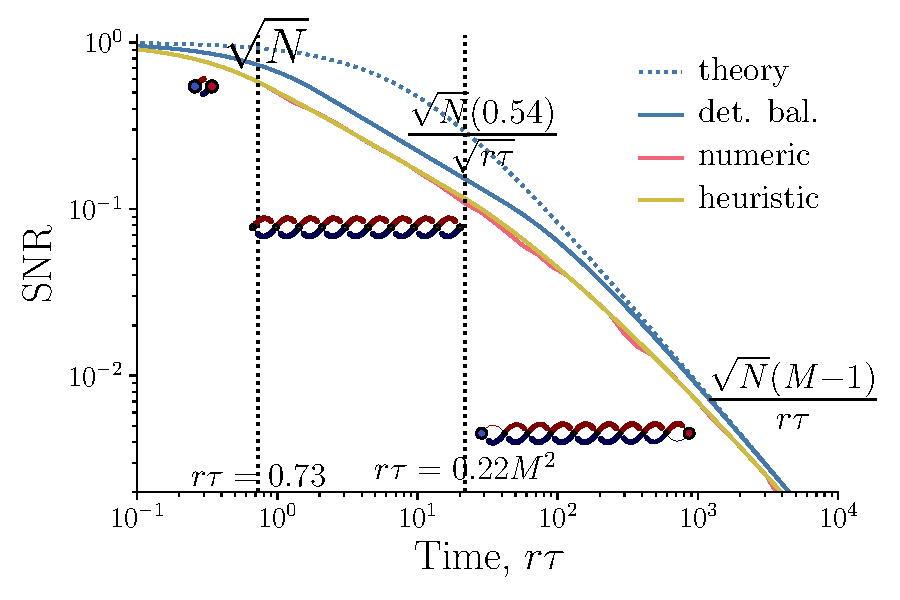
\includegraphics[width=0.8\linewidth]{LenvHeuristic.pdf}\\
  \caption[Heuristic envelope for the signal-to-noise ratio]
  {Heuristic envelope  for the signal-to-noise ratio, \cref{eq:henv}.
  Analytic expressions from \cref{eq:henvapprox} are only valid to the right of each region.}\label{fig:heuristicenv}
\end{figure}

%================================================================================

\section{Conclusions}\label{sec:conclusions}


We do not expect to find precisely these models inside real synapses.
First, evolution was faced with stronger constraints than us when designing these synapses as it had to build them out of real molecules.
Second, the set of priorities faced by evolution would have been longer than just performance in recognition memory at a single timescale.

Nevertheless, the qualitative message of our findings should be more robust to reality:
%
\begin{itemize}
  \item \emph{Short} timescale \(\to\) \emph{intermediate} timescales: transition topology goes from \\ short and wide \(\to\) long and thin.
  \item \emph{Intermediate} timescale \(\to\) \emph{long} timescales: transition probabilities go from \\ strong and deterministic \(\to\) weak and stochastic.
\end{itemize}
%
This is what we expect to find in the different brain regions that store memories for different timescales.

The transition between the two regimes is set by the maximum number of states, \(M\) (we can't set the number of states to be exactly \(M\), as bigger models can always mimic smaller models).
So, if we want to lengthen the timescale at which a synapse is optimal, we start by adding extra states, using the topology mechanism.
When we run out of states, we switch to the stochasticity mechanism and make the end states sticky.
The stochasticity mechanism is only used when we no longer have the option of using the topology mechanism.
It is always better to add more states, if allowed, than to make transitions stochastic.

We can get some insight into why this is by considering a serial model with \(M\) states and all transition topologies equal to \(q\).
%
\begin{equation*}
\begin{aligned}
  \snr(0) &\propto q,
  &\qquad
  \max_a \tau_a &\propto \frac{1}{q}, \\
  \snr(0) &\propto \frac{1}{M},
  &\qquad
  \max_a \tau_a &\propto M^2. \\
\end{aligned}
\end{equation*}
%
The initial SNR scales as described because it is related to the equilibrium probability flux between the weak and strong states, and the equilibrium distribution is uniform over \(M\) states.
The lifetime scales as described because \(rq\) sets the timescale for transitions, and for diffusion distance (\(M\)) scales as the square root of time.

If we want to lengthen the lifetime with a fixed hit on initial SNR, we get a larger increase by increasing \(M\) than by decreasing \(q\).
If we want to lengthen the lifetime by a fixed amount, we take a smaller hit on initial SNR by increasing \(M\) than by decreasing \(q\).
Thus, we always get more bang for our buck using the topology mechanism than the stochasticity mechanism.


%\subsection*{Acknowledgements}



%%%%%%%%%%%%%%%%%%%%%%%%%%%%%%%%%%%%%%%%%%%%%%%%%%%%%%%%%%%%%%%%%%%%%%%%%%
%\subsection*{Appendices}
%\appendix
%%%%%%%%%%%%%%%%%%%%%%%%%%%%%%%%%%%%%%%%%%%%%%%%%%%%%%%%%%%%%%%%%%%%%%%%%%





%%%%%%%%%%%%%%%%%%%%%%%%%%%%%%%%%%%%%%%%%%%%%%%%%%%%%%%%%%%%%%%%%%%%%%%%%%

\bibliographystyle{utcaps_sl}
\bibliography{maths,neuro,markov}

\end{document}
